%%=============================================================================
%% LaTeX sjabloon voor bachelorproef, HoGent Bedrijf en Organisatie
%% Opleiding Toegepaste Informatica
%%=============================================================================

\documentclass[fleqn,a4paper,12pt]{book}

%%=============================================================================
%% LaTeX sjabloon voor de bachelorproef, HoGent Bedrijf en Organisatie
%% Opleiding toegepaste informatica
%%
%% Structuur en algemene vormgeving. Meestal hoef je hier niets te wijzigen.
%%
%% Vormgeving gebaseerd op "The Legrand Orange Book", version 2.0 (9/2/15)
%% door Mathias Legrand (legrand.mathias@gmail.com) met aanpassingen door
%% Vel (vel@latextemplates.com). Het oorspronkelijke template is te vinden op
%% http://www.LaTeXTemplates.com
%%
%% Aanpassingen voor HoGent toegepaste informatica: 
%%   Bert Van Vreckem <bert.vanvreckem@hogent.be>
%% Licentie: 
%%   CC BY-NC-SA 3.0 (http://creativecommons.org/licenses/by-nc-sa/3.0/)
%%=============================================================================

%%-----------------------------------------------------------------------------
%% Packages
%%-----------------------------------------------------------------------------

\usepackage[top=3cm,bottom=3cm,left=3cm,right=3cm,headsep=10pt,a4paper]{geometry} % Page margins
\usepackage[utf8]{inputenc}  % Accenten gebruiken in tekst (vb. é ipv \'e)
\usepackage{amsfonts}        % AMS math packages: extra wiskundige
\usepackage{amsmath}         %   symbolen (o.a. getallen-
\usepackage{amssymb}         %   verzamelingen N, R, Z, Q, etc.)
\usepackage[english,dutch]{babel}    % Taalinstellingen: woordsplitsingen,
                             %  commando's voor speciale karakters
                             %  ("dutch" voor NL)
\usepackage{iflang}
\usepackage{eurosym}         % Euro-symbool €
\usepackage{geometry}
\usepackage{graphicx}        % Invoegen van tekeningen
\graphicspath{{img/}}       % Specifies the directory where pictures are stored
\usepackage{tikz}            % Required for drawing custom shapes
\usepackage[pdftex,bookmarks=true]{hyperref}
                             % PDF krijgt klikbare links & verwijzingen,
                             %  inhoudstafel
\usepackage{enumitem}        % Customize lists
\setlist{nolistsep}         % Reduce spacing between list items
\usepackage{listings}        % Broncode mooi opmaken
\usepackage{multirow}        % Tekst over verschillende cellen in tabellen
\usepackage{rotating}        % Tabellen en figuren roteren

\usepackage{booktabs}        % Required for nicer horizontal rules in tables
\usepackage{siunitx}

\usepackage{xcolor}          % Required for specifying colors by name
\definecolor{maincolor}{RGB}{0,147,208} % Define the main color used for 
                             % highlighting throughout the book
                             % 0, 147, 208 = officiële kleur HoGent FBO

% Paragraph style: no indent, add space between paragraphs
\setlength{\parindent}{0em}
\setlength{\parskip}{1em}

\usepackage{etoolbox}
\usepackage{titling} % Macros for title, author, etc
\usepackage{lipsum}          % Voor vultekst (lorem ipsum)

\usepackage[acronym]{glossaries} % Voor glossary en acronyms

%----------------------------------------------------------------------------------------
%	FONTS
%----------------------------------------------------------------------------------------

\usepackage{avant} % Use the Avantgarde font for headings
%\usepackage{times} % Use the Times font for headings
\usepackage{mathptmx} % Use the Adobe Times Roman as the default text font together with math symbols from the Sym­bol, Chancery and Com­puter Modern fonts

\usepackage{microtype} % Slightly tweak font spacing for aesthetics
\usepackage[utf8]{inputenc} % Required for including letters with accents
\usepackage[T1]{fontenc} % Use 8-bit encoding that has 256 glyphs

%------------------------------------------------------------------------------
%	TITLE PAGE
%------------------------------------------------------------------------------

\newcommand{\inserttitlepage}{%
\begin{titlepage}
  \newgeometry{top=2cm,bottom=1.5cm,left=1.5cm,right=1.5cm}
  \begin{center}

    \begingroup
    \rmfamily
    
\includegraphics[width=2.5cm]{img/HG-beeldmerk-woordmerk}\\[.5cm]
    Faculteit Bedrijf en Organisatie\\[3cm]
    \titel
    \vfill
    \student\\[3.5cm]
    Scriptie voorgedragen tot het bekomen van de graad van\\professionele bachelor in de toegepaste informatica\\[2cm]
    Promotor:\\
    \promotor\\
    \ifdefempty{\copromotor}{\vspace{2.5cm}}{Co-promotor:\\\copromotor\\[2.5cm]}
    Instelling: \instelling\\[.5cm]
    Academiejaar: \academiejaar\\[.5cm]
    \ifcase \examenperiode \or Eerste \or Tweede \else Derde \fi examenperiode
    \endgroup

  \end{center}
  \restoregeometry
\end{titlepage}
  \emptypage
\begin{titlepage}
  \newgeometry{top=5.35cm,bottom=1.5cm,left=1.5cm,right=1.5cm}
  \begin{center}

    \begingroup
    \rmfamily
    \IfLanguageName{dutch}{Faculteit Bedrijf en Organisatie}{Faculty of Business and Information Management}\\[3cm]
    \titel
    \vfill
    \student\\[3.5cm]
    \IfLanguageName{dutch}{Scriptie voorgedragen tot het bekomen van de graad van\\professionele bachelor in de toegepaste informatica}{Thesis submitted in partial fulfilment of the requirements for the degree of\\professional bachelor of applied computer science}\\[2cm]
    Promotor:\\
    \promotor\\
    \ifdefempty{\copromotor}{\vspace{2.5cm}}{Co-promotor:\\\copromotor\\[2.5cm]}
    \IfLanguageName{dutch}{Instelling}{Institution}: \instelling\\[.5cm]
    \IfLanguageName{dutch}{Academiejaar}{Academic year}: \academiejaar\\[.5cm]
    \IfLanguageName{dutch}{%
    \ifcase \examenperiode \or Eerste \or Tweede \else Derde \fi examenperiode}{%
    \ifcase \examenperiode \or First \or Second \else Third \fi examination period}
    \endgroup

  \end{center}
  \restoregeometry
\end{titlepage}
}

%----------------------------------------------------------------------------------------
%	BIBLIOGRAPHY AND INDEX
%----------------------------------------------------------------------------------------

\usepackage[style=apa,backend=biber]{biblatex}
\usepackage{csquotes}
\DeclareLanguageMapping{dutch}{dutch-apa}
\addbibresource{bachproef-tin.bib} % BibTeX bibliography file
\addbibresource{../voorstel/voorstel.bib}
\defbibheading{bibempty}{}

\usepackage{calc} % For simpler calculation - used for spacing the index letter headings correctly
\usepackage{makeidx} % Required to make an index
\makeindex % Tells LaTeX to create the files required for indexing

%----------------------------------------------------------------------------------------
%	MAIN TABLE OF CONTENTS
%----------------------------------------------------------------------------------------

\usepackage{titletoc} % Required for manipulating the table of contents

\contentsmargin{0cm} % Removes the default margin

% Part text styling
\titlecontents{part}[0cm]
{\addvspace{20pt}\centering\large\bfseries}
{}
{}
{}

% Chapter text styling
\titlecontents{chapter}[1.25cm] % Indentation
{\addvspace{12pt}\large\sffamily\bfseries} % Spacing and font options for chapters
{\color{maincolor!60}\contentslabel[\Large\thecontentslabel]{1.25cm}\color{maincolor}} % Chapter number
{\color{maincolor}}
{\color{maincolor!60}\normalsize\;\titlerule*[.5pc]{.}\;\thecontentspage} % Page number

% Section text styling
\titlecontents{section}[1.25cm] % Indentation
{\addvspace{3pt}\sffamily\bfseries} % Spacing and font options for sections
{\contentslabel[\thecontentslabel]{1.25cm}} % Section number
{}
{\hfill\color{black}\thecontentspage} % Page number
[]

% Subsection text styling
\titlecontents{subsection}[1.25cm] % Indentation
{\addvspace{1pt}\sffamily\small} % Spacing and font options for subsections
{\contentslabel[\thecontentslabel]{1.25cm}} % Subsection number
{}
{\ \titlerule*[.5pc]{.}\;\thecontentspage} % Page number
[]

% List of figures
\titlecontents{figure}[0em]
{\addvspace{-5pt}\sffamily}
{\thecontentslabel\hspace*{1em}}
{}
{\ \titlerule*[.5pc]{.}\;\thecontentspage}
[]

% List of tables
\titlecontents{table}[0em]
{\addvspace{-5pt}\sffamily}
{\thecontentslabel\hspace*{1em}}
{}
{\ \titlerule*[.5pc]{.}\;\thecontentspage}
[]

%----------------------------------------------------------------------------------------
%	MINI TABLE OF CONTENTS IN PART HEADS
%----------------------------------------------------------------------------------------

% Chapter text styling
\titlecontents{lchapter}[0em] % Indenting
{\addvspace{15pt}\large\sffamily\bfseries} % Spacing and font options for chapters
{\color{maincolor}\contentslabel[\Large\thecontentslabel]{1.25cm}\color{maincolor}} % Chapter number
{}
{\color{maincolor}\normalsize\sffamily\bfseries\;\titlerule*[.5pc]{.}\;\thecontentspage} % Page number

% Section text styling
\titlecontents{lsection}[0em] % Indenting
{\sffamily\small} % Spacing and font options for sections
{\contentslabel[\thecontentslabel]{1.25cm}} % Section number
{}
{}

% Subsection text styling
\titlecontents{lsubsection}[.5em] % Indentation
{\normalfont\footnotesize\sffamily} % Font settings
{}
{}
{}

%----------------------------------------------------------------------------------------
%	PAGE HEADERS
%----------------------------------------------------------------------------------------

\usepackage{fancyhdr} % Required for header and footer configuration

\pagestyle{fancy}
\renewcommand{\chaptermark}[1]{\markboth{\sffamily\normalsize\bfseries\chaptername\ \thechapter.\ #1}{}} % Chapter text font settings
\renewcommand{\sectionmark}[1]{\markright{\sffamily\normalsize\thesection\hspace{5pt}#1}{}} % Section text font settings
\fancyhf{} \fancyhead[LE,RO]{\sffamily\normalsize\thepage} % Font setting for the page number in the header
\fancyhead[LO]{\rightmark} % Print the nearest section name on the left side of odd pages
\fancyhead[RE]{\leftmark} % Print the current chapter name on the right side of even pages
\renewcommand{\headrulewidth}{0.5pt} % Width of the rule under the header
\addtolength{\headheight}{2.5pt} % Increase the spacing around the header slightly
\renewcommand{\footrulewidth}{0pt} % Removes the rule in the footer
\fancypagestyle{plain}{\fancyhead{}\renewcommand{\headrulewidth}{0pt}} % Style for when a plain pagestyle is specified

% Removes the header from odd empty pages at the end of chapters
\makeatletter
\renewcommand{\cleardoublepage}{
\clearpage\ifodd\c@page\else
\hbox{}
\vspace*{\fill}
\thispagestyle{empty}
\newpage
\fi}

%----------------------------------------------------------------------------------------
%	THEOREM STYLES
%----------------------------------------------------------------------------------------

\usepackage{amsmath,amsfonts,amssymb,amsthm} % For math equations, theorems, symbols, etc

\newcommand{\intoo}[2]{\mathopen{]}#1\,;#2\mathclose{[}}
\newcommand{\ud}{\mathop{\mathrm{{}d}}\mathopen{}}
\newcommand{\intff}[2]{\mathopen{[}#1\,;#2\mathclose{]}}
\newtheorem{notation}{Notation}[chapter]

% Boxed/framed environments
\newtheoremstyle{maincolornumbox}% % Theorem style name
{0pt}% Space above
{0pt}% Space below
{\normalfont}% % Body font
{}% Indent amount
{\small\bf\sffamily\color{maincolor}}% % Theorem head font
{\;}% Punctuation after theorem head
{0.25em}% Space after theorem head
{\small\sffamily\color{maincolor}\thmname{#1}\nobreakspace\thmnumber{\@ifnotempty{#1}{}\@upn{#2}}% Theorem text (e.g. Theorem 2.1)
\thmnote{\nobreakspace\the\thm@notefont\sffamily\bfseries\color{black}---\nobreakspace#3.}} % Optional theorem note
\renewcommand{\qedsymbol}{$\blacksquare$}% Optional qed square

\newtheoremstyle{blacknumex}% Theorem style name
{5pt}% Space above
{5pt}% Space below
{\normalfont}% Body font
{} % Indent amount
{\small\bf\sffamily}% Theorem head font
{\;}% Punctuation after theorem head
{0.25em}% Space after theorem head
{\small\sffamily{\tiny\ensuremath{\blacksquare}}\nobreakspace\thmname{#1}\nobreakspace\thmnumber{\@ifnotempty{#1}{}\@upn{#2}}% Theorem text (e.g. Theorem 2.1)
\thmnote{\nobreakspace\the\thm@notefont\sffamily\bfseries---\nobreakspace#3.}}% Optional theorem note

\newtheoremstyle{blacknumbox} % Theorem style name
{0pt}% Space above
{0pt}% Space below
{\normalfont}% Body font
{}% Indent amount
{\small\bf\sffamily}% Theorem head font
{\;}% Punctuation after theorem head
{0.25em}% Space after theorem head
{\small\sffamily\thmname{#1}\nobreakspace\thmnumber{\@ifnotempty{#1}{}\@upn{#2}}% Theorem text (e.g. Theorem 2.1)
\thmnote{\nobreakspace\the\thm@notefont\sffamily\bfseries---\nobreakspace#3.}}% Optional theorem note

% Non-boxed/non-framed environments
\newtheoremstyle{maincolornum}% % Theorem style name
{5pt}% Space above
{5pt}% Space below
{\normalfont}% % Body font
{}% Indent amount
{\small\bf\sffamily\color{maincolor}}% % Theorem head font
{\;}% Punctuation after theorem head
{0.25em}% Space after theorem head
{\small\sffamily\color{maincolor}\thmname{#1}\nobreakspace\thmnumber{\@ifnotempty{#1}{}\@upn{#2}}% Theorem text (e.g. Theorem 2.1)
\thmnote{\nobreakspace\the\thm@notefont\sffamily\bfseries\color{black}---\nobreakspace#3.}} % Optional theorem note
\renewcommand{\qedsymbol}{$\blacksquare$}% Optional qed square
\makeatother

% Defines the theorem text style for each type of theorem to one of the three styles above
\newcounter{dummy}
\numberwithin{dummy}{section}
\theoremstyle{maincolornumbox}
\newtheorem{theoremeT}[dummy]{Theorem}
\newtheorem{problem}{Problem}[chapter]
\newtheorem{exerciseT}{Exercise}[chapter]
\theoremstyle{blacknumex}
\newtheorem{exampleT}{Example}[chapter]
\theoremstyle{blacknumbox}
\newtheorem{vocabulary}{Vocabulary}[chapter]
\newtheorem{definitionT}{Definition}[section]
\newtheorem{corollaryT}[dummy]{Corollary}
\theoremstyle{maincolornum}
\newtheorem{proposition}[dummy]{Proposition}

%----------------------------------------------------------------------------------------
%	DEFINITION OF COLORED BOXES
%----------------------------------------------------------------------------------------

\RequirePackage[framemethod=default]{mdframed} % Required for creating the theorem, definition, exercise and corollary boxes

% Theorem box
\newmdenv[skipabove=7pt,
skipbelow=7pt,
backgroundcolor=black!5,
linecolor=maincolor,
innerleftmargin=5pt,
innerrightmargin=5pt,
innertopmargin=5pt,
leftmargin=0cm,
rightmargin=0cm,
innerbottommargin=5pt]{tBox}

% Exercise box
\newmdenv[skipabove=7pt,
skipbelow=7pt,
rightline=false,
leftline=true,
topline=false,
bottomline=false,
backgroundcolor=maincolor!10,
linecolor=maincolor,
innerleftmargin=5pt,
innerrightmargin=5pt,
innertopmargin=5pt,
innerbottommargin=5pt,
leftmargin=0cm,
rightmargin=0cm,
linewidth=4pt]{eBox}

% Definition box
\newmdenv[skipabove=7pt,
skipbelow=7pt,
rightline=false,
leftline=true,
topline=false,
bottomline=false,
linecolor=maincolor,
innerleftmargin=5pt,
innerrightmargin=5pt,
innertopmargin=0pt,
leftmargin=0cm,
rightmargin=0cm,
linewidth=4pt,
innerbottommargin=0pt]{dBox}

% Corollary box
\newmdenv[skipabove=7pt,
skipbelow=7pt,
rightline=false,
leftline=true,
topline=false,
bottomline=false,
linecolor=gray,
backgroundcolor=black!5,
innerleftmargin=5pt,
innerrightmargin=5pt,
innertopmargin=5pt,
leftmargin=0cm,
rightmargin=0cm,
linewidth=4pt,
innerbottommargin=5pt]{cBox}

% Creates an environment for each type of theorem and assigns it a theorem text style from the "Theorem Styles" section above and a colored box from above
\newenvironment{theorem}{\begin{tBox}\begin{theoremeT}}{\end{theoremeT}\end{tBox}}
\newenvironment{exercise}{\begin{eBox}\begin{exerciseT}}{\hfill{\color{maincolor}\tiny\ensuremath{\blacksquare}}\end{exerciseT}\end{eBox}}
\newenvironment{definition}{\begin{dBox}\begin{definitionT}}{\end{definitionT}\end{dBox}}
\newenvironment{example}{\begin{exampleT}}{\hfill{\tiny\ensuremath{\blacksquare}}\end{exampleT}}
\newenvironment{corollary}{\begin{cBox}\begin{corollaryT}}{\end{corollaryT}\end{cBox}}

%----------------------------------------------------------------------------------------
%	REMARK ENVIRONMENT
%----------------------------------------------------------------------------------------

\newenvironment{remark}{\par\vspace{10pt}\small % Vertical white space above the remark and smaller font size
\begin{list}{}{
\leftmargin=35pt % Indentation on the left
\rightmargin=25pt}\item\ignorespaces % Indentation on the right
\makebox[-2.5pt]{\begin{tikzpicture}[overlay]
\node[draw=maincolor!60,line width=1pt,circle,fill=maincolor!25,font=\sffamily\bfseries,inner sep=2pt,outer sep=0pt] at (-15pt,0pt){\textcolor{maincolor}{R}};\end{tikzpicture}} % Orange R in a circle
\advance\baselineskip -1pt}{\end{list}\vskip5pt} % Tighter line spacing and white space after remark

%----------------------------------------------------------------------------------------
%	SECTION NUMBERING IN THE MARGIN
%----------------------------------------------------------------------------------------

\makeatletter
\renewcommand{\@seccntformat}[1]{\llap{\textcolor{maincolor}{\csname the#1\endcsname}\hspace{1em}}}
\renewcommand{\section}{\@startsection{section}{1}{\z@}
{-4ex \@plus -1ex \@minus -.4ex}
{1ex \@plus.2ex }
{\normalfont\large\sffamily\bfseries}}
\renewcommand{\subsection}{\@startsection {subsection}{2}{\z@}
{-3ex \@plus -0.1ex \@minus -.4ex}
{0.5ex \@plus.2ex }
{\normalfont\sffamily\bfseries}}
\renewcommand{\subsubsection}{\@startsection {subsubsection}{3}{\z@}
{-2ex \@plus -0.1ex \@minus -.2ex}
{.2ex \@plus.2ex }
{\normalfont\small\sffamily\bfseries}}
\renewcommand\paragraph{\@startsection{paragraph}{4}{\z@}
{-2ex \@plus-.2ex \@minus .2ex}
{.1ex}
{\normalfont\small\sffamily\bfseries}}

%----------------------------------------------------------------------------------------
%	PART HEADINGS
%----------------------------------------------------------------------------------------

% numbered part in the table of contents
\newcommand{\@mypartnumtocformat}[2]{%
\setlength\fboxsep{0pt}%
\noindent\colorbox{maincolor!20}{\strut\parbox[c][.7cm]{\ecart}{\color{maincolor!70}\Large\sffamily\bfseries\centering#1}}\hskip\esp\colorbox{maincolor!40}{\strut\parbox[c][.7cm]{\linewidth-\ecart-\esp}{\Large\sffamily\centering#2}}}%
%%%%%%%%%%%%%%%%%%%%%%%%%%%%%%%%%%
% unnumbered part in the table of contents
\newcommand{\@myparttocformat}[1]{%
\setlength\fboxsep{0pt}%
\noindent\colorbox{maincolor!40}{\strut\parbox[c][.7cm]{\linewidth}{\Large\sffamily\centering#1}}}%
%%%%%%%%%%%%%%%%%%%%%%%%%%%%%%%%%%
\newlength\esp
\setlength\esp{4pt}
\newlength\ecart
\setlength\ecart{1.2cm-\esp}
\newcommand{\thepartimage}{}%
\newcommand{\partimage}[1]{\renewcommand{\thepartimage}{#1}}%
\def\@part[#1]#2{%
\ifnum \c@secnumdepth >-2\relax%
\refstepcounter{part}%
\addcontentsline{toc}{part}{\texorpdfstring{\protect\@mypartnumtocformat{\thepart}{#1}}{\partname~\thepart\ ---\ #1}}
\else%
\addcontentsline{toc}{part}{\texorpdfstring{\protect\@myparttocformat{#1}}{#1}}%
\fi%
\startcontents%
\markboth{}{}%
{\thispagestyle{empty}%
\begin{tikzpicture}[remember picture,overlay]%
\node at (current page.north west){\begin{tikzpicture}[remember picture,overlay]%
\fill[maincolor!20](0cm,0cm) rectangle (\paperwidth,-\paperheight);
\node[anchor=north] at (4cm,-3.25cm){\color{maincolor!40}\fontsize{220}{100}\sffamily\bfseries\@Roman\c@part};
\node[anchor=south east] at (\paperwidth-1cm,-\paperheight+1cm){\parbox[t][][t]{8.5cm}{
\printcontents{l}{0}{\setcounter{tocdepth}{1}}%
}};
\node[anchor=north east] at (\paperwidth-1.5cm,-3.25cm){\parbox[t][][t]{15cm}{\strut\raggedleft\color{white}\fontsize{30}{30}\sffamily\bfseries#2}};
\end{tikzpicture}};
\end{tikzpicture}}%
\@endpart}
\def\@spart#1{%
\startcontents%
\phantomsection
{\thispagestyle{empty}%
\begin{tikzpicture}[remember picture,overlay]%
\node at (current page.north west){\begin{tikzpicture}[remember picture,overlay]%
\fill[maincolor!20](0cm,0cm) rectangle (\paperwidth,-\paperheight);
\node[anchor=north east] at (\paperwidth-1.5cm,-3.25cm){\parbox[t][][t]{15cm}{\strut\raggedleft\color{white}\fontsize{30}{30}\sffamily\bfseries#1}};
\end{tikzpicture}};
\end{tikzpicture}}
\addcontentsline{toc}{part}{\texorpdfstring{%
\setlength\fboxsep{0pt}%
\noindent\protect\colorbox{maincolor!40}{\strut\protect\parbox[c][.7cm]{\linewidth}{\Large\sffamily\protect\centering #1\quad\mbox{}}}}{#1}}%
\@endpart}
\def\@endpart{\vfil\newpage
\if@twoside
\if@openright
\null
\thispagestyle{empty}%
\newpage
\fi
\fi
\if@tempswa
\twocolumn
\fi}

%----------------------------------------------------------------------------------------
%	CHAPTER HEADINGS
%----------------------------------------------------------------------------------------

% A switch to conditionally include a picture, implemented by  Christian Hupfer
\newif\ifusechapterimage
\usechapterimagetrue
\newcommand{\thechapterimage}{}%
\newcommand{\chapterimage}[1]{\ifusechapterimage\renewcommand{\thechapterimage}{#1}\fi}%
\def\@makechapterhead#1{%
{\parindent \z@ \raggedright \normalfont
\ifnum \c@secnumdepth >\m@ne
\if@mainmatter
\begin{tikzpicture}[remember picture,overlay]
\node at (current page.north west)
{\begin{tikzpicture}[remember picture,overlay]
\node[anchor=north west,inner sep=0pt] at (0,0) {\ifusechapterimage\includegraphics[width=\paperwidth]{\thechapterimage}\fi};
\draw[anchor=west] (\Gm@lmargin,-9cm) node [line width=2pt,rounded corners=15pt,draw=maincolor,fill=white,fill opacity=0.5,inner sep=15pt]{\strut\makebox[22cm]{}};
\draw[anchor=west] (\Gm@lmargin+.3cm,-9cm) node {\huge\sffamily\bfseries\color{black}\thechapter. #1\strut};
\end{tikzpicture}};
\end{tikzpicture}
\else
\begin{tikzpicture}[remember picture,overlay]
\node at (current page.north west)
{\begin{tikzpicture}[remember picture,overlay]
\node[anchor=north west,inner sep=0pt] at (0,0) {\ifusechapterimage\includegraphics[width=\paperwidth]{\thechapterimage}\fi};
\draw[anchor=west] (\Gm@lmargin,-9cm) node [line width=2pt,rounded corners=15pt,draw=maincolor,fill=white,fill opacity=0.5,inner sep=15pt]{\strut\makebox[22cm]{}};
\draw[anchor=west] (\Gm@lmargin+.3cm,-9cm) node {\huge\sffamily\bfseries\color{black}#1\strut};
\end{tikzpicture}};
\end{tikzpicture}
\fi\fi\par\vspace*{270\p@}}}

%-------------------------------------------

\def\@makeschapterhead#1{%
\begin{tikzpicture}[remember picture,overlay]
\node at (current page.north west)
{\begin{tikzpicture}[remember picture,overlay]
\node[anchor=north west,inner sep=0pt] at (0,0) {\ifusechapterimage\includegraphics[width=\paperwidth]{\thechapterimage}\fi};
\draw[anchor=west] (\Gm@lmargin,-9cm) node [line width=2pt,rounded corners=15pt,draw=maincolor,fill=white,fill opacity=0.5,inner sep=15pt]{\strut\makebox[22cm]{}};
\draw[anchor=west] (\Gm@lmargin+.3cm,-9cm) node {\huge\sffamily\bfseries\color{black}#1\strut};
\end{tikzpicture}};
\end{tikzpicture}
\par\vspace*{270\p@}}
\makeatother

%----------------------------------------------------------------------------------------
%	HYPERLINKS IN THE DOCUMENTS
%----------------------------------------------------------------------------------------

\usepackage{hyperref}
\hypersetup{hidelinks,backref=true,pagebackref=true,hyperindex=true,colorlinks=false,breaklinks=true,urlcolor= maincolor,bookmarks=true,bookmarksopen=false,pdftitle={Title},pdfauthor={Author}}
\usepackage{bookmark}
\bookmarksetup{
open,
numbered,
addtohook={%
\ifnum\bookmarkget{level}=0 % chapter
\bookmarksetup{bold}%
\fi
\ifnum\bookmarkget{level}=-1 % part
\bookmarksetup{color=maincolor,bold}%
\fi
}
}

%----------------------------------------------------------------------------------------
%	Java source code
%----------------------------------------------------------------------------------------

% Commando voor invoegen Java-broncodebestanden (dank aan Niels Corneille)
% Gebruik:
%   \codefragment{source/MijnKlasse.java}{Uitleg bij de code}
%
% Je kan dit aanpassen aan de taal die je zelf het meeste gebruikt in je
% bachelorproef.
\newcommand{\codefragment}[3]{ \lstset{%
  language=[Sharp]C,
  breaklines=true,
  float=th,
  caption={#2},
  basicstyle=\scriptsize,
  frame=single,
  extendedchars=\true
}
\lstinputlisting{#1}
\label{#3}}



% Leeg blad
\newcommand{\emptypage}{%
\newpage
\thispagestyle{empty}
\mbox{}
\newpage
}


\newglossaryentry{latex}
{
        name=latex,
        description={Is a mark up language specially suited for 
scientific documents}
}
 
\newglossaryentry{maths}
{
        name=mathematics,
        description={Mathematics is what mathematicians do}
}
 
\newglossaryentry{formula}
{
        name=formula,
        description={A mathematical expression}
}
\newacronym{xr}{XR}{Extended Reality}
\newacronym{vr}{VR}{Virtual Reality}
\newacronym{ar}{AR}{Augmented Reality}
\newacronym{mr}{MR}{Mixed Reality}
\newacronym{hmd}{HMD}{Head Mounted Display}
\newacronym{slam}{SLAM}{Simultaneous localization and mapping}
\newacronym{3dof}{3DOF}{Three degrees of freedom}
\newacronym{6dof}{6DOF}{Six degrees of freedom}
\newacronym{dof}{DOF}{Degrees of Freedom}
\newacronym{fov}{FoV}{Field-Of-View}
\newacronym{imu}{IMU}{Inertial Measurement Unit}
\newacronym{muhka}{MuHKA}{Museum voor Hedendaagse Kunst Antwerpen}

\makeglossaries


%%---------- Documenteigenschappen --------------------------------------------
%% TODO: Vul dit aan met je eigen info:

% Je eigen naam
\newcommand{\student}{Matthias De Fré}

% De naam van je promotor (lector van de opleiding)
\newcommand{\promotor}{Jens Buysse}

% De naam van je co-promotor. Als je promotor ook je opdrachtgever is en je
% dus ook inhoudelijk begeleidt (en enkel dan!), mag je dit leeg laten.
\newcommand{\copromotor}{Joris De Lamper}

% Indien je bachelorproef in opdracht van/in samenwerking met een bedrijf of
% externe organisatie geschreven is, geef je hier de naam. Zoniet laat je dit
% zoals het is.
\newcommand{\instelling}{---}

% De titel van het rapport/bachelorproef
\newcommand{\titel}{Kan AR / VR gebruiker worden om het levensverhaal van een persoon te vertellen in musea}

% Datum van indienen (gebruik telkens de deadline, ook al geef je eerder af)
\newcommand{\datum}{31 mei 2019}

% Academiejaar
\newcommand{\academiejaar}{2018-2018}

% Examenperiode
%  - 1e semester = 1e examenperiode => 1
%  - 2e semester = 2e examenperiode => 2
%  - tweede zit  = 3e examenperiode => 3
\newcommand{\examenperiode}{2}

%%=============================================================================
%% Inhoud document
%%=============================================================================

\begin{document}

%---------- Taalselectie ------------------------------------------------------
% Als je je bachelorproef in het Engels schrijft, haal dan onderstaande regel
% uit commentaar. Let op: de tekst op de voorkaft blijft in het Nederlands, en
% dat is ook de bedoeling!

%\selectlanguage{english}

%---------- Titelblad ---------------------------------------------------------
\inserttitlepage

%---------- Samenvatting, voorwoord -------------------------------------------
\usechapterimagefalse
%%=============================================================================
%% Voorwoord
%%=============================================================================

\chapter*{Woord vooraf}
\label{ch:voorwoord}

%% TODO:
%% Het voorwoord is het enige deel van de bachelorproef waar je vanuit je
%% eigen standpunt (``ik-vorm'') mag schrijven. Je kan hier bv. motiveren
%% waarom jij het onderwerp wil bespreken.
%% Vergeet ook niet te bedanken wie je geholpen/gesteund/... heeft


%%=============================================================================
%% Samenvatting
%%=============================================================================

% TODO: De "abstract" of samenvatting is een kernachtige (~ 1 blz. voor een
% thesis) synthese van het document.
%
% Deze aspecten moeten zeker aan bod komen:
% - Context: waarom is dit werk belangrijk?
% - Nood: waarom moest dit onderzocht worden?
% - Taak: wat heb je precies gedaan?
% - Object: wat staat in dit document geschreven?
% - Resultaat: wat was het resultaat?
% - Conclusie: wat is/zijn de belangrijkste conclusie(s)?
% - Perspectief: blijven er nog vragen open die in de toekomst nog kunnen
%    onderzocht worden? Wat is een mogelijk vervolg voor jouw onderzoek?
%
% LET OP! Een samenvatting is GEEN voorwoord!

%%---------- Nederlandse samenvatting -----------------------------------------
%
% TODO: Als je je bachelorproef in het Engels schrijft, moet je eerst een
% Nederlandse samenvatting invoegen. Haal daarvoor onderstaande code uit
% commentaar.
% Wie zijn bachelorproef in het Nederlands schrijft, kan dit negeren, de inhoud
% wordt niet in het document ingevoegd.

\IfLanguageName{english}{%
\selectlanguage{dutch}
\chapter*{Samenvatting}
\lipsum[1-4]
\selectlanguage{english}
}{}

%%---------- Samenvatting -----------------------------------------------------
% De samenvatting in de hoofdtaal van het document

\chapter*{\IfLanguageName{dutch}{Samenvatting}{Abstract}}


%---------- Inhoudstafel ------------------------------------------------------
\pagestyle{empty} % No headers
\tableofcontents % Print the table of contents itself
\cleardoublepage % Forces the first chapter to start on an odd page so it's on the right
\pagestyle{fancy} % Print headers again

%---------- Lijst figuren, afkortingen, ... -----------------------------------

% Indien gewenst kan je hier een lijst van figuren/tabellen opgeven. Geef in
% dat geval je figuren/tabellen altijd een korte beschrijving:
%
%  \caption[korte beschrijving]{uitgebreide beschrijving}

\listoffigures
\listoftables

% Als je een lijst van afkortingen of termen wil toevoegen, dan hoort die
% hier thuis. Gebruik bijvoorbeeld de ``glossaries'' package.
% https://www.sharelatex.com/learn/Glossaries
\printglossary
\printglossary[type=\acronymtype]

%%---------- Kern -------------------------------------------------------------

%%=============================================================================
%% Inleiding
%%=============================================================================

\chapter{Inleiding}
\label{ch:inleiding}

\section{Probleemstelling}
\label{sec:probleemstelling}

Vele musea organiseren tentoonstellingen rond bekende (historische) personen. Deze tentoonstellingen zijn echter vaak verouderd en evolueren ook niet echt mee met technologische ontwikkelingen. Musea die wel de nieuwste technologische snufjes gebruiken moeten vaak terugvallen op standaardapplicaties die vaak niet specifiek genoeg zijn. Deze studie wil één van deze specifieke use cases (het vertellen van een levensverhaal) oplossen door een lijst op te stellen van de mogelijkheden, met hun voor- en nadelen, die musea hebben om dit te implementeren. Alhoewel de hoofddoelgroep musea met deze use case zijn, probeert de studie een zo'n ruim mogelijk beeld te schetsen van de verschillende mogelijkheden om virtual reality te implementeren in een museum zodat deze lijst ook bruikbaar is voor musea met soortgelijke use cases.

\section{Onderzoeksvraag}
\label{sec:onderzoeksvraag}

\begin{enumerate}
    \item 'Op welke manieren kan virtual reality worden geïmplementeerd in musea?' geeft aan welke technologieën een museum allemaal kan gebruiken om \acrshort{vr} te implementeren.
    \item 'Hoe kan het levensverhaal van een persoon worden verteld in musea en welke technologie is het meest gepast' gebruikt de meeste passende technologie uit de eerste onderzoeksvraag om zo de mogelijkheden van deze technologie te verwerken in een applicatie.
    \item 'Wat is het beste framework van de gekozen technologie op basis van verschillende factoren, beschreven in hoofdstuk \ref{ch:methodologie}' 
\end{enumerate}

\section{Onderzoeksdoelstelling}
\label{sec:onderzoeksdoelstelling}

Het resultaat van dit onderzoek is een longlist die musea kunnen gebruiken als handleiding om te weten wat de voor- en nadelen zijn van verschillende \acrshort{vr} technologieën. Alsook is er een voorbeeld van een applicatie die een antwoord geeft op de tweede onderzoeksvraag.

\section{Opzet van deze bachelorproef}
\label{sec:opzet-bachelorproef}

% Het is gebruikelijk aan het einde van de inleiding een overzicht te
% geven van de opbouw van de rest van de tekst. Deze sectie bevat al een aanzet
% die je kan aanvullen/aanpassen in functie van je eigen tekst.

De rest van deze bachelorproef is als volgt opgebouwd:

In Hoofdstuk~\ref{ch:stand-van-zaken} wordt een overzicht gegeven van de stand van zaken binnen het onderzoeksdomein, op basis van een literatuurstudie.

In Hoofdstuk~\ref{ch:longlist} wordt een lijst gegeven van verschillende technologieën die gebruikt kunnen worden om \acrshort{vr} te implementeren en beantwoordt dus de eerste onderzoeksvraag.

In Hoofdstuk~\ref{ch:shortlist} wordt een lijst gegeven van verschillende frameworks over de gekozen technologie uit de longlist en bevat voor elk van deze frameworks een score om zo een antwoord te geven op de tweede onderzoeksvraag.

In Hoofdstuk~\ref{ch:methodologie} wordt de methodologie toegelicht en worden de gebruikte onderzoekstechnieken besproken om een antwoord te kunnen formuleren op het experiment van de derde onderzoeksvraag.

In Hoofdstuk~\ref{ch:experiment} worden de resultaten van het experiment geanalyseerd en besproken.

In Hoofdstuk~\ref{ch:experiment} wordt het prototype van de beste technologie besproken, alsook de ontwikkeling van dit prototype wordt hier besproken.

In Hoofdstuk~\ref{ch:conclusie} tenslotte wordt de conclusie gegeven en een antwoord geformuleerd op de onderzoeksvragen. Daarbij wordt ook een aanzet gegeven voor toekomstig onderzoek binnen dit domein.


\chapter{Stand van zaken}
\label{ch:stand-van-zaken}

% Tip: Begin elk hoofdstuk met een paragraaf inleiding die beschrijft hoe
% dit hoofdstuk past binnen het geheel van de bachelorproef. Geef in het
% bijzonder aan wat de link is met het vorige en volgende hoofdstuk.

% Pas na deze inleidende paragraaf komt de eerste sectiehoofding.

% TODO CONTENT Inleiding
% TODO Verwijderen template text
Door de recente opkomst van nieuwe virtual reality applicaties denken veel mensen dat VR een nieuwe technologie is. Alhoewel dat de exacte oorsprong van VR moeilijk te achterhalen is omdat er geen vaste definitie van bestaat, kan één van de eerste commerciële toepassingen gevonden worden in 1939, namelijk de View-Master. Gebruikers konden door dit apparaat kijken om zo full-screen panorama's te zien van locaties in de wereld. Een ander voorbeeld is de Sensorama van (INSERT CITE). Deze machine had de mogelijkheid om een video af te spelen en ondertussen de zintuigen van de gebruiker te stimuleren. Dit was mogelijk door geuren, wind en bewegingen na te bootsen.
\begin{figure}
    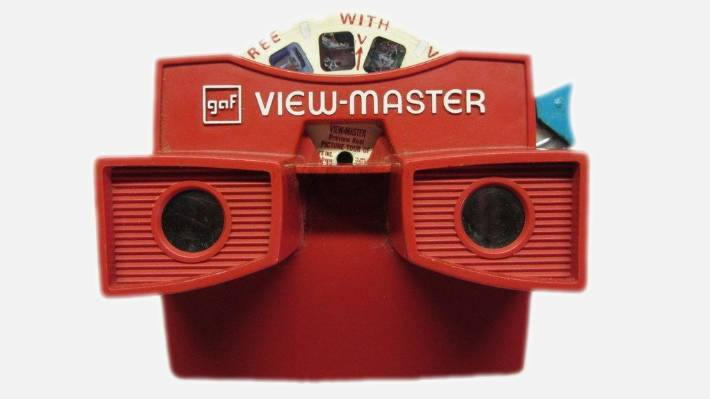
\includegraphics[width=\linewidth]{viewmaster.jpg}
    \caption{De View-Master, uitgebracht in 1939}
    \label{fig:viewmaster}
\end{figure}

\begin{figure}
    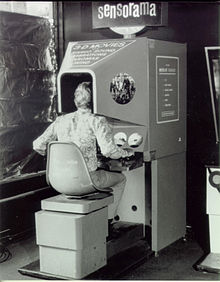
\includegraphics[width=\linewidth]{sensorama.jpg}
    \caption{De Sensorama}
    \label{fig:sensorama}
\end{figure}

\section{Teleprescence}
Tijdens het gebruik van een VR applicatie is gebruiker aanwezig in 2 "werelden" tegelijk, teleprescence is dus dat de gebruiker zich meer aanwezig voelt in de virtuele wereld dan de fysieke wereld.
Een grote fout die veel mensen maken is Virtual Reality koppelen aan hardware terwijl dit veel meer dan dit is \autocite{Steuer1992}.
% TODO CONTENT Perceptie van automatische en gecontrolleerde mentale processen

Teleprescence komt niet alleen voor bij VR maar bij elke applicatie waarbij die een communicatie medium gebruikt. Dit medium is niet alleen digitaal ook fysieke zaken zoals kranten kan je het gevoel geven dat je er echt 'aanwezig' bent, mensen ervaren dit soms als rillingen wanneer ze bijvoorbeeld iets choquerend lezen. 
Een groot verschil tussen VR en de andere mediums waarbij teleprescence in meespeelt is dat bij VR de gebruiker beide zender en ontvanger is. Hij zal acties versturen naar de virtuele wereld en beelden terugkrijgen op basis van zijn acties.
Aan de hand van deze definitie kunnen we dus afleiden dat zelfs 360 graden video's ook als VR tellen. Dit is omdat de beelden die de gebruiker te zien krijgt afhangen van de draaihoek hoe hij kijkt naar het scherm, zelfs telefoneren kan men eigenlijk zien als VR \autocite{Steuer1992}.
Omdat deze definitie van VR heel ruim is beperkt deze bachelorproef zich tot de technologieën die gebruiken maken van een gyroscoop of andere sensoren om zo een betere ervaring te geven.

% TODO TRANSLATE Immersive
Om het niveau van teleprescence te verhogen bij de gebruiker zijn volgende twee variabelen belangrijk: de immersive / echtheid en de interactiviteit van de applicatie \autocite{Steuer1992}.
De belangrijkste factor die de echtheid van een applicatie verhoogt is de stimulatie van de zintuigen. Wanneer de gebruiker bijvoorbeeld echt de wind en het water voelt terwijl hij in een virtuele regen staat zal hij misschien meer geneigd zijn om de virtuele wereld als echt te gaan ervaren \autocite{Steuer1992}. De invloed van deze externe factoren kan afhangen van gebruiker tot gebruiker, sommige gebruikers staan hier meer voor open en zullen zich sneller ondergedompeld voelen in de ervaring dan anderen.
Voor het verhogen van interactiviteit zijn er verscheidene mogelijkheden, de gekozen manier zal vaak afhangen van de gekozen technologie. Een \acrfull{hmd} implementeert dit door de gebruiker beide handen te laten gebruiken om acties uit te voeren. Deze acties kunnen dan gebeuren door het herkennen van de lichaamsdelen of door externe controllers.

Het herkennen van een een lichaamsdeel komt voor wanneer de software effectief het lichaamsdeel zelf herkent en niet a.h.v. sensoren bevestigd op het lichaamsdeel. Om gebruik te maken van deze techniek is er wel een camera nodig die bevestigd is aan de voorkant van het apparaat (HoloLens, Smartphone) of een externe camera die lichaamsdelen herkent, bijvoorbeeld Microsoft Kinect \autocite{Ren2013}.
Meestal zal een applicatie de vorm van een hand proberen te detecteren, a.h.v. deze vorm kan dan een 'gesture' worden herkent die dan gelinkt is aan een bepaalde actie \autocite{Piumsomboon2013}. 
Voor het herkennen van gestures is er de mogelijkheid om computer vision te gebruiken \autocite{Ji2013}.


Alhoewel deze twee variabelen een grote rol spelen bij teleprescence is er het doel van de applicatie ook zeer belangrijk. Een goed voorbeeld hiervan is Pokémon GO. Bij het bestuderen van de implementatie van de twee variabelen hierbij ziet men het volgende. De interactiviteit van de app is redelijk simpel, de spelers lopen rond in de echte wereld door hun gps te gebruiken en kunnen zo op het scherm een beweging doen om monsters te vangen. Realisme is dan geïmplementeerd door gebruik te maken van augmented reality, deze plaatst dan de monsters in de echte wereld. Zoals er te zien is zijn deze twee implementaties niet zo geavanceerd en kwamen ze al voor in andere apps (Ingress), maar toch is Pokémon GO veel succesvoller dan deze andere apps. Dit komt vooral omdat Pokémon GO voldoet aan de verwachte ervaring van de gebruiker, namelijk een echte trainer zijn zoals in de Pokémon games en serie \autocite{Tang2017}. Hieruit volgt dus de conclusie dat de graad waarop deze variabelen zijn geïmplementeerd zal afhangen van de use case. Ook speelde het sociale aspect een grote rol in het continue succes van Pokémon GO, dit kan dus ook als een mogelijke invloed gezien worden waar er rekening mee moet worden gehouden \autocite{Tang2017}.


Het is dus voor deze reden dat deze studie een derde variabele toevoegt, namelijk de bruikbaarheid voor de gekozen use case. Net zoals in bij de 2 variabelen van \textcite{Steuer1992} bestaat deze uit 3 subcategorieën namelijk: praktisch, financieel en logisch. Aan de hand van de 2 voorafgaande variabelen en deze nieuwe wordt er in de longlist bepaald welke technologie er verder besproken a.h.v. een shortlist met verschillende frameworks. 

\section{Computer Vision}

% TODO CONTENT Computer Vision
Vooral bij Augmented of Mixed Reality zal men te maken krijgen met computer vision. Computer vision is interdisciplinair wetenschappelijk gebied dat verschillende domeinen bevat in verband met herkenning a.h.v. beeldmateriaal. Waaronder: herkennen van objecten, afbeeldingen, bewegingen maar ook het aanpassen van beelden om zo ruis te verwijderen valt hieronder (INSERT CITE).

Voor vele van deze algoritmen maken gebruik van artificiële intelligentie, een vaak gebruikte techniek hiervoor is 'convolutional neural network' \autocite{Ji2013}. Afhankelijk van het algoritme zal dit neuraal netwerk opzoek gaan naar features die nuttig zijn. Bij gezichtsherkenning is het vinden van de neus, ogen en randen van het gezicht belangrijk terwijl een automatische drone eerder wilt weten waar de obstakels zich bevinden. Met de gevonden features kan de applicatie dan het gezicht blijven volgen en een filter hierop toepassen of kan er een 3d object worden gemaakt (bijvoorbeeld een obstakel) in het geval van de drone. 

Het gebruik van computer vision wordt later verder besproken in de secties \ref{sec:augmentedreality} en \ref{sec:mixedreality}. % TODO (Mixed Reality => Spatial Mapping ²²² Augmented Reality => Image detection / ground detection)
% TODO CITE referentie naar site https://hackernoon.com/building-a-facial-recognition-pipeline-with-deep-learning-in-tensorflow-66e7645015b8
\begin{figure}
    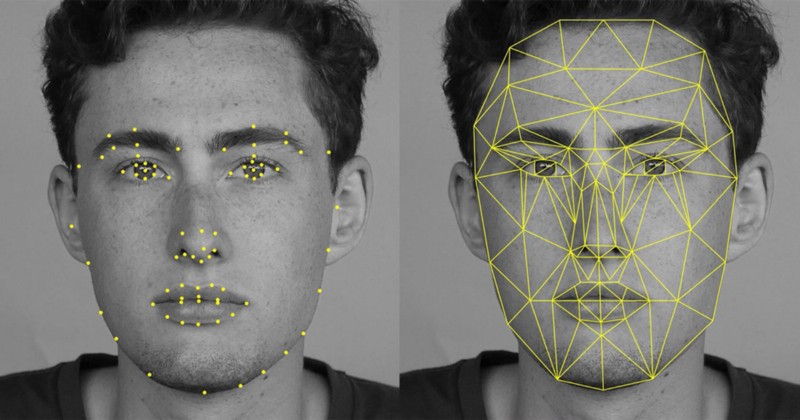
\includegraphics[width=\linewidth]{cnnFace.jpeg}
    \caption{Herkennen van features om zo een digitaal gezicht te maken}
    \label{fig:cnnface}
\end{figure}

\section{Degrees Of Freedom}

VR technologieën kunnen ook nog eens worden onderverdeeld afhankelijk van het aantal vrijheidsgraden dat ze ondersteunen. In de wereld van VR komen \acrshort{3dof} en \acrshort{6dof} het meeste voor. Deze vrijheidsgraden bepalen in welke mate de gebruiker kan bewegen in de virtuele wereld \autocite{Chen1995}.

% TODO TRANSLATE yaw, pitch, rol
\acrshort{3dof} ondersteunt alleen rotationele bewegingen, deze zijn: yaw, pitch en rol. Deze kunnen hebben echter alleen maar de mogelijkheid om de camera te draaien en niet van locatie veranderen. Bij 6DOF zijn is dit wel mogelijk omdat deze over volgende bewegingen beschikt: up and down, front and back en left and right.
Een technologie met 6DOF heeft wel de mogelijkheid om in de virtuele wereld rond te lopen, alsook zal de mogelijkheid er nog altijd zijn om te camera te draaien omdat 6DOF beschikt over rotationale en positionele bewegingen. De ondersteuning van deze vrijheidsgraden ligt niet alleen bij de technologie zelf maar ook bij de gebruikte hardware \autocite{Chen1995}. In de longlist zal er in detail worden besproken hoeveel vrijheidsgraden ondersteund zijn en welke hardware er juist nodig is om te gebruiken.

\begin{figure}
    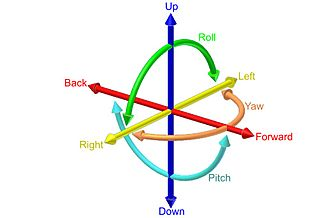
\includegraphics[width=\linewidth]{dof.jpg}
    \caption{\acrfull{6dof}}
    \label{fig:dof}
\end{figure}

% TODO CONTENT Uitleg IMU
% TODO CONTENT Uitleg odementry => hier of bij AR / MR

\section{Gelijkaardige use cases}
% TODO CONTENT Gelijkaardige use case
% TODO ASK Plaatsen na computer vision? Maakt gebruik van image scanning.
\subsection{Cleveland Museum of Art}
Dit museum maakt gebruik van software genaamd ArtLens. Artlens bestaat uit verschillende onderdelen die gebundeld zijn in 1 dezelfde smartphone app. Met deze app kunnen bezoekers een interactieve tour krijgen. In het museum bevinden zich bluetooth beacons waardoor de app kan weten waar de bezoeker zich bevind en zo tonen waar het volgende kunstwerk is. Ook kan de gebruiker zijn interesses opgeven waardoor de app voorstellen kan doen van kunstwerken die dichtbij zijn. 
De bezoekers kunnen ook zelf hun eigen tours maken en deze delen met andere gebruikers wat dan weer het sociale aspect van de applicatie bevordert.

Het VR gedeelte van deze applicatie vindt plaats wanneer een gebruiker met zijn camera op een schilderij mikt. Hierbij zal er dan op het scherm, via augmented reality, extra informatie komen over het schilderij.
In het museum bevinden zich ook terminals waar de gebruikers hun smartphone op kunnen leggen. Hierdoor verschijnt er op een groot scherm een opdracht die dan moet worden uitgevoerd bijvoorbeeld het nadoen van een schilderij of na een tijdje het schilderij zo goed mogelijk proberen natekenen \autocite{Ding2017}.

\subsection{Smithsonian}
Bij het Smithsonian wordt er ook gebruikgemaakt augmented reality, deze keer door gebruik te maken van BroadcastAR. Deze software gebruikt een camera om zo te streamen naar een groot scherm waar de bezoekers dan de AR-objecten kunnen zien. Het nadeel van deze implementatie is dat er weinig of geen interactie is tussen de gebruiker en de software. 

Het Smithsonian heeft ook nog een tweede augemented reality app waarbij gebruikers hun camera kunnen richten op skeletten om zo het skelet om te toveren naar een model van het levend dier.

\subsection{Historium Brugge}
Het Historium in Brugge maakt geen gebruik van augemented reality maar wel van virtual reality. De applicatie bied twee soorten ervaringen aan, City VR en Historium VR. Bij City VR kan de gebruiker verschillende locaties van Brugge bezoeken in VR terwijl hij bij Historium VR een interactive rondeleiding krijgt over het middeleeuwse Brugge. Bij City VR applicatie kan worden geïnstalleerd op elke smartphone die AR ondersteund, voor Historium VR is er echter wel een VR headset inclusief controllers nodig. 

% \lipsum[7-20]

% %%=============================================================================
%% Methodologie
%%=============================================================================

\chapter{Methodologie van het Experiment}
\label{ch:methodologie}

Om de kwaliteit van een augmented reality framework te beoordelen is het experiment in twee delen opgedeeld. Het eerste deel van het experiment zal gaan over hoe goed de frameworks de core van de applicatie kunnen implementeren. Elk framework zal dezelfde lijst met tien images. De bedoeling is dat elk framework zoveel mogelijk images probeert te herkennen. De gebruikte lijst met images kan u vinden in de bijlage. De lijst is opgebouwd uit vijf makkelijke afbeeldingen en vijf moeilijkere afbeeldingen. Om te weten wat een moeilijke of makkelijke afbeelding is gebruikt deze studie volgende criteria.

\begin{itemize}
    \item Veel features
    \item Geen repetitieve features
    \item Goed contrast
\end{itemize} 


Het tweede deel van het experiment zal gaan over de performance van elk framework. Dit wordt gedaan door FPS, RAM gebruik en batterij verbruik met elkaar te vergelijken. Omdat ieder framework gebruik maakt van andere API's moet voor elk van deze een soortgelijke applicatie worden voorzien. Deze applicatie zal een afbeelding herkennen aan hierop een 3d object tonen. Bij het klikken op dit object zal dit veranderen in een ander object. Het is de bedoeling dat bij het verliezen van de tracking van de afbeelding, en hierna terug tracken, het nieuwe object er nog steeds is en niet terug verandert is naar het oude.
%% TODO: Hoe ben je te werk gegaan? Verdeel je onderzoek in grote fasen, en
%% licht in elke fase toe welke stappen je gevolgd hebt. Verantwoord waarom je
%% op deze manier te werk gegaan bent. Je moet kunnen aantonen dat je de best
%% mogelijke manier toegepast hebt om een antwoord te vinden op de
%% onderzoeksvraag.

\chapter{Longlist verschillende AR / VR technologieën}
\label{ch:longlist}

Hierin worden de verschillende technologieën overlopen die kunnen gebruikt worden om deze use case te volbrengen.
Elke sectie bevat de belangrijkste zaken in verband met de technologie waaronder: gebruikte algoritmen, zaken waar men rekening mee moet houden, sensoren en een analyse over de de drie variabelen (realisme, interactiviteit, bruikbaarheid).

\section{Head Mounted Virtual Reality}
Head mounted virtual reality maakt gebruik van een \acrshort{hmd} die de gebruiker op zijn hoofd zet. Deze headset zal dan een virtuele wereld tonen die volledig aangestuurd is door de applicatie zelf. Deze wereld zal dus geen rekening houden met de echte wereld, dit kan hierdoor wel voor problemen zorgen indien er geen sensor of camera aanwezig is die je tegenhoud om tegen muren te lopen.

HMD kan over \acrshort{3dof} of \acrshort{6dof} beschikken afhankelijk van de gebruikte headset. De 3DOF headsets zijn wel goedkoper dan de \acrshort{6dof} en maken vaak gebruik van de smartphone om zo het beeld te kunnen tonen. 
% TODO CONTENT Iets over het beeld dat in 2 wordt gesplitst, op elke oog 1 beeld
% TODO ASK Is uitleg over hoe het beeld op de ogen wordt geprojecteerd en geinterpreteerd door de hersenen teveel of topic?
\subsection{Medische Klachten}
Sommige mensen kunnen bij het gebruik van een HDM ziek of misselijk worden. De oorzaak van dit is meestal verbonden met een te klein of onnatuurlijk gezichtsveld, \acrfull{fov} (INSERT CITE) of als de beweging in de applicatie gebeurt a.h.v. teleportatie. (INSERT CITE) Deze teleportatie beweging komt vooral voor bij \acrshort{3dof} omdat hierbij er manieren zijn om de camerea te bewegen, namelijk teleportatie of via een joystick.

De tijd tussen de beweging in de echte wereld en de virtuele (latency) kan ook invloed hebben op virtual reality sickness indien deze te hoog is \autocite{Elbamby2018} en \autocite{DiZio2000}. 
% TODO TRANSLATE disconnection
Veel van deze problemen hebben te maken met de staat van de huidige hardware en hoe deze geen hogere FoV aan een hoge framerate kunnen ondersteunen. Een hoge en stabiele framerate is nodig indien om de gebruiker een aangename ervaring te geven. Een te lage framerate kan ervoor zorgen dat er (TRANSLATE) disconnection is tussen de beweging van de gebruiker en het gene dat effectief op het scherm gebeurt, dit kan voor frustratie zorgen.
\subsection{Sensoren}
% TODO ASK Extra uitleg over IMU of niet?
De gebruikte sensoren bij een \acrshort{hmd} hangen af van de gewenste bewegingen. Als er alleen maar rotationale bewegingen nodig zijn zal een gyroscoop of een \acrfull{imu} (bij standalone headsets) genoeg zijn om zo de yaw, pitch, roll te kunnen meten en hierop te kunnen reageren \autocite{LaValle2014}. Indien er ook positionale bewegingen nodig zijn zal de kamer wel moeten beschikken over infraroodsensoren om zo de headset te kunnen tracken. Deze sensoren zorgen er wel voor dat er meer voorbereiding nodig is alvorens het gebruik van de headset.
% TODO CITE Infrared
\subsection{Realisme}
Omdat de headset het beeld op de beide ogen projecteert is er geen besef van de echte wereld en kan de virtuele wereld makkelijker als 'echt' worden ervaart. De headset zal ook gemonteerd zijn op het hoofd waardoor beide handen vrij zijn om acties uit te voeren. Hierdoor maken beide handen deel uit van de virtuele wereld wat de ervaring nog meer realistischer maakt.
% TODO CONTENT Iets over latency => tijd tussen beweging hoofd en beweging in vr
\subsection{Interactiviteit}
De manier waarop de gebruiker zal interageren met de virtuele wereld zal afhangen van het aantal vrijheidsgraden bij \acrshort{6dof} zal hij de mogelijkheid hebben om zelf te kunnen rondlopen in de wereld terwijl bij \acrshort{3dof} dit a.h.v. een joystick of via teleportatie zal moeten. Er is ook altijd de mogelijkheid om controllers te gebruiken. Deze controllers zullen dan de mogelijkheid bieden om fysieke interacties te kunnen doen, bijvoorbeeld het oppakken van een virtueel object of door op één van de knoppen van de controller te duwen een actie uit te voeren.

\begin{figure}
    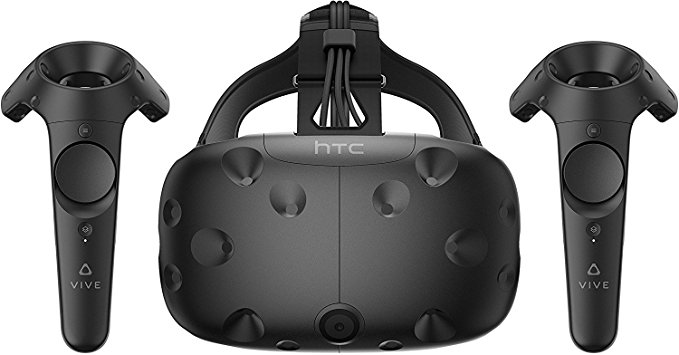
\includegraphics[width=\linewidth]{headset.jpg}
    \caption{HTC Vive headset en controllers}
    \label{fig:htcvive}
\end{figure}

\subsection{Bruikbaarheid}
De bruikbaarheid van HMD in musea is nogal laag. Het is niet echt praktisch om gebruikers met een \acrshort{hmd} (Google Cardboard of Full HMD) te laten rondlopen omdat dit veel ruimte in het museum zou kosten om goed te implementeren. Gebruikt het museum dit toch kan er hierbij toch een hoge financiele kost aanhangen. Afhankelijk of de gebruikers moeten langskomen voor de applicatie uit te proberen of niet kan het zijn dat het museum headsets moet aankopen en hiervoor een speciale ruimte moet inrichten.

Meeste mensen die naar een museum gaan willen juist rondlopen in het museum zelf en niet in de virtuele versie hiervan. Het is daarom ook niet echt logisch om een HMD hiervoor te gebruiken. Natuurlijk als het museum een ervaring zoals bij het Historium Brugge wilt is een \acrshort{hmd} wel gepast of zelfs nodig.

\section{Augmented Reality} \label{sec:augmentedreality}
Augmented reality kan het best worden omschreven als het plaatsen van virtuele objecten in de echte wereld maar zonder de mogelijkheid om fysiek te reageren met deze objecten. Voor deze technologie is er vaak geen headset nodig maar eerder gewoon een smartphone. Indien toch gewenst, of nodig, is wel de mogelijkheid om een augmented reality headset te gebruiken. Deze bieden de mogelijkheid om de smartphone in te plaatsen waardoor deze zal functioneren als het hardwaregedeelte van de bril. \autocite{Schops2014}.

\subsection{Plane Detection}
Om virtuele objecten in de echte wereld te kunnen plaatsen moet de echte wereld eerst gemapped. Dit gebeurt a.h.v. computer vision om zo te weten waar een nieuwe plane begint en eindigt. Dit algoritme zal constant lopen om zo nieuwe planes te kunnen ontdekken \autocite{Xu2018}. Het gebruikte algoritme zal een vorm zijn van odometry tracking.

Eens een plane ontdekt is kan deze dienen als een platform om nieuwe objecten op te plaatsen. De applicatie zal dan het object verbinden aan een ankerpunt (INSERT CITE). Het object verbindt zich dan met een ankerpunt waar deze zijn locatie zal onthouden zelfs als de gebruiker wat verder weg wandelend. Er zijn echter wel limieten aan dit anker, indien de gebruiker te ver weggaat van het punt en nadien terugkomt zal het virtuele object verplaatst zijn, dit begrip noemt drifting \autocite{You1999}. Indien er grote precisie nodig is voor de applicatie kan dit wel problemen zorgen.

\subsection{Odometry Tracking}

Door gebruik te maken van de \acrshort{imu} en dus ook de gyroscope en accelerometers die in een smartphone zitten heeft deze de mogelijkheid om vlakken te herkennen maar ook om zo achteraf terug te kunnen weten welke gebieden er al gescand zijn geweest. \autocite{Leutenegger2015}.

De twee grote native AR frameworks maken hier beide gebruik van. De techniek die ARCore gebruikt noemt 'concurrent odometry and mapping' (INSERT CITE GOOGLE) terwijl de gebruikte techniek van ARKit 'visual-inertial odometry' (INSERT CITE APPLE) noemt. 

Beide technieken werken echter wel op dezelfde manier. Het algoritme combineert de motion data van de smartphone met de herkende features van het camerabeeld en berekent zo de verandering in positie. Hierdoor kunnen de juiste anchors en dus hun objecten worden getoond (INSERT CITE APPLE) (INSERT CITE GOOGLE).

Een iets oudere vorm van odometry tracking is \acrfull{slam}, deze zal ook gebruik maken van features maar is eerder gericht om een kaart bij te houden van de gemapte omgeving. Dit gebeurt door te weten wanneer een bepaalde gebied al ontdekt is en wanneer het dus niet nodig is om deze opnieuw toe te voegen aan de mapping (loop closure). Hierdoor zal \acrshort{slam} wel een beter globaal beeld hebben de ruimte in tegenstelling tot odometry tracking, Deze is meer gericht op het behouden van het lokaal beeld zodat de objecten goed op hun plaats blijven \autocite{Yousif2015}. Dit is echter wel niet toepasbaar op elk framework omdat deze meestal een combinatie van de twee gebruiken of een eigen implementatie.

\begin{figure}
    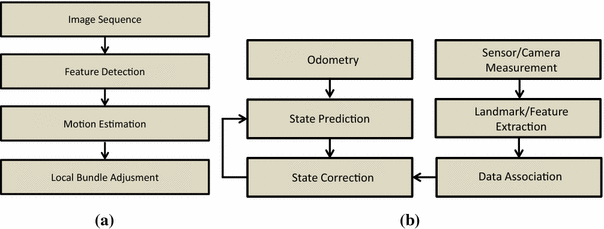
\includegraphics[width=\linewidth]{voVSslam.png}
    \caption{Visual Odometry versus SLAM \autocite{Yousif2015}}
    \label{fig:voVSslam}
\end{figure}


De kwaliteit van het camerabeeld zal een invloed hebben op de accuraatheid van het algoritme. Als er bijvoorbeeld te weinig licht is zal het algoritme de locatie niet kunnen herkennen. (INSERT CITE APPLE).

\begin{figure}
    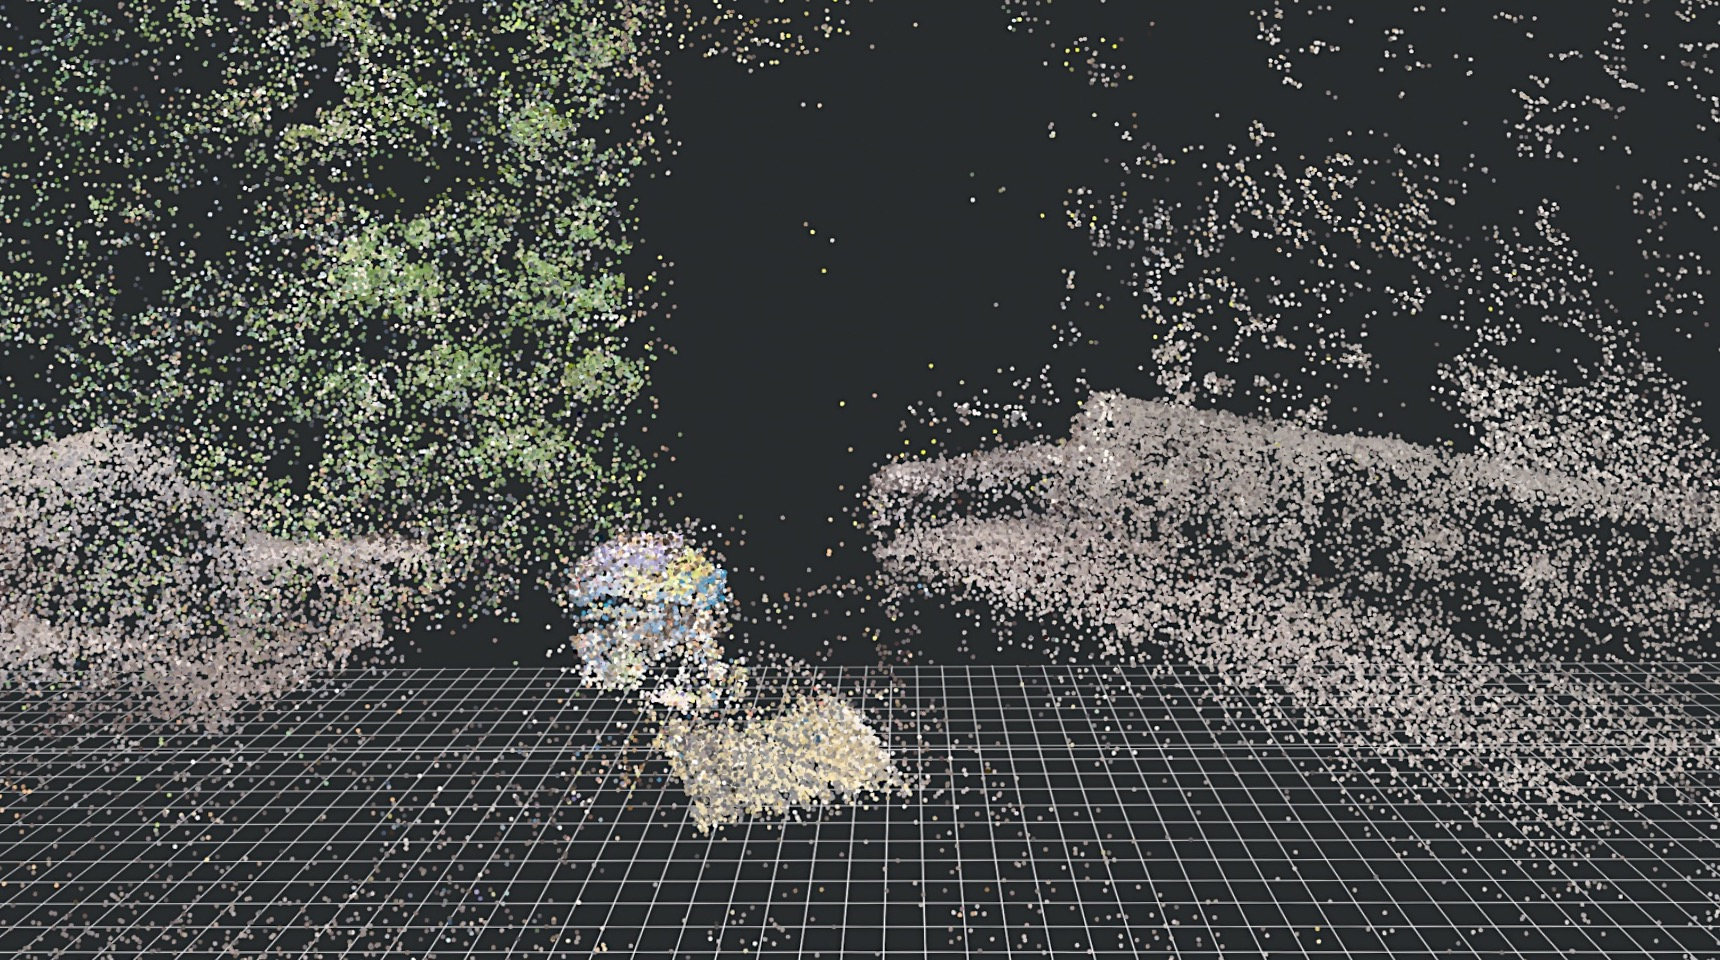
\includegraphics[width=\linewidth]{pointcloudarkit.jpg}
    \caption{ARKit Visual-Inertial Odometry}
    \label{fig:pointcloudarkit}
\end{figure}


% TODO IMAGE Point cloud / plane detection
% TODO CITE Object Anchor, alleen maar concrete implementaties gevonden ARCORE / ARKIT https://developers.google.com/ar/develop/developer-guides/anchors
\subsection{Image Recognition}
Een tweede manier om virtuele objecten in de wereld te plaatsen is met image recognition. Meeste frameworks zullen ook hiervoor computer vision gebruiken zoals te zien op figuur \ref{fig:imagereg}.

De image zal dienen als ankerpunt om de virtuele objecten op te plaatsen en te onthouden. 
Eens de image is herkend is er de mogelijkheid om de objecten te erop plaatsen. Wanneer de smartphone de afbeelding niet meer kan zien zal deze de positie van het object, na een tijdje, vergeten en zal tracking zich uitzetten. Het virtuele object verschijnt terug wanneer de smartphone de afbeelding weer herkent.

Een alternatief van image recognition is object recognition. In plaats van het herkennen van een 2d afbeelding wordt er hier een 3d object gebruikt (INSERT CITE VUFORIA).

\begin{figure}
    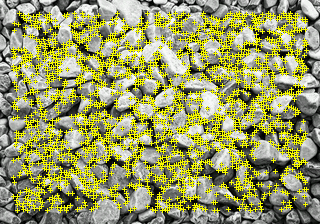
\includegraphics[width=\linewidth]{vuforiaImageReg.png}
    \caption{Aangeduide features op een afbeelding}
    \label{fig:imagereg}
\end{figure}

\subsection{Realisme}
Omdat augmented reality geen besef heeft van aanpassingen in de wereld, bv een persoon die voor de camera loopt is het soms wel moeilijk om een immersieve ervaring te maken. Dit is vooral omdat de huidige hardware van een smartphone het niet aankan om constant op zoek te gaan naar kleine veranderingen terwijl een HoloLens (Mixed Reality) dit bijvoorbeeld wel kan.

Er zijn wel nog extra technieken die frameworks kunnen gebruiken om toch nog wat extra immersie te creëren zoals light estimation. Bij dit kunnen virtuele objecten reageren wanneer de echte wereld lichter of donkerder wordt (INSERT CITE GOOGLE).

\subsection{Interactiviteit}
Het gebruik van een smartphone kan de interactiviteit van een applicatie verminderen omdat de gebruiker deze moet vasthouden en dus maar één hand vrij heeft. Door gebruik te maken van een augmented reality headset zal dit probleem zich wel oplossen.

De virtuele wereld zal wel nooit echt reageren op fysieke handelingen wat er dus voor zorgt dat elke actie op het scherm van de smartphone moet gebeuren.

Alhoewel deze twee zaken als grote nadelen kunnen gezien worden kan men hier ook gebruik van maken. Aangezien de smartphone in de hand is kunnen ook niet augmented reality zaken worden gebruikt. Er kan bijvoorbeeld een menu zijn waar de gebruiker verschillende rondleidingen uit kan kiezen.

\subsection{Bruikbaarheid}
Het gebrek aan een kabel bij augmented reality zorgt er voor dat dit op vele plaatsen bruikbaar is. Vooral bij musea is dit handig omdat het hele museum kan dienen als platform voor de virtuele wereld en er geen speciale ruimtes nodig zijn.

Vele mensen die naar musea gaan hebben vaak hun smartphone bij wat er dus voor zorgt dat de gebruiker alleen een app nodig heeft om mee te doen aan de ervaring.

Image en object recognition is ook iets dat heel makkelijk te implementeren is in musea omdat bestaande kunstwerken kunnen dienen als objecten voor het weergeven van de virtuele content.

\section{360 Degrees Videos}
360 Degrees Videos is de simpelste vorm van virtual reality in deze longlist. Eigenlijk zijn dit gewoon videos waarbij de gebruiker de camera 360 graden kan draaien \autocite{Hosseini2016}.

Om deze video's te bekijken is er eigenlijk niets speciaal nodig. Als een 360 graden video op een desktop wordt bekeken zal de camera nog altijd kunnen draaien door middel van de pijltjestoetsen. Terwijl wanneer deze op een apparaat met een \acrshort{imu} zal draaien door met het apparaat te bewegen. Wanneer er een IMU wordt gebruikt kan er nog altijd een onderscheid tussen een \acrshort{hmd} en een gewoon apparaat. Als een \acrshort{hmd} aanwezig zal de video worden getoond in VR. Bij een gewoon device zal de video echter een normale video zijn maar wel met de mogelijkheid om de camera te draaien.

\subsection{Recording}
Het opnemen van deze video is wel iets ingewikkelder. Er zijn twee formaten om een 360 graden video voor te stellen namelijk equirectangular en cubic \autocite{Lee2010}. 

Bij het equirectangular formaat zal deze elke frame van de video op een vlakke afbeelding projecteren. Deze afbeelding kan dan op een bol worden gelegd en deze bol zal de video voorstellen. Een makkelijke manier om een equirectangular afbeelding voor te stellen is namelijk een wereldkaart. Wanneer men een wereldkaart op een bol legt zal deze een wereldbol worden.
 
\begin{figure}
    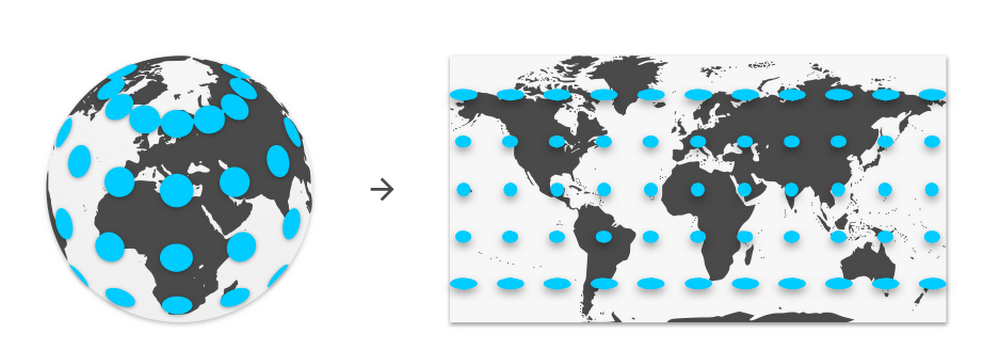
\includegraphics[width=\linewidth]{equirectangular.png}
    \caption{Een equirectangular projectie van de wereld}
    \label{fig:equirectangularprojection}
\end{figure}

Het cubic formaat werkt ongeveer op dezelfde manier behalve dat deze de frame in zes afbeeldingen zal opdelen die elk een zijde van de kubus zal voorstellen.

% TODO ASK Uitleg van projectie op vlakke afbeelding?
\subsection{Realisme}
Een 360 graden video kan bestaan uit echte beelden of virtuele beelden op die manier zijn er veel mogelijkheden om deze video immersief te maken. 

Wanneer men kijkt naar de sensorama kan men zien dat dit eigenlijk ook een 360 graden video is. Hier werd de ervaring immersief gemaakt door de zintuigen te stimuleren en zoals al eerder vermeld is dit één van de belangrijkste manieren waarop het gevoel van realisme kan worden opgewekt.

\subsection{Interactiviteit}
Het enigste wat een gebruiker kan doen bij een 360 graden video is het ronddraaien van de camera hierdoor is de interactiviteit minimaal. Toch zijn er 360 apps die net iets meer interactiviteit hebben, bij deze is er bijvoorbeeld de mogelijkheid om naar objecten te kijken en daarover informatie te tonen. Ook is er de mogelijkheid om voorwerpen te verstoppen in de video waar de gebruiker dan op zoek naar moet gaan.
\subsection{Bruikbaarheid}
Omdat de video op elk apparaat dat Youtube of een andere 360 player ondersteund kan draaien is het heel bruikbaar. Echter om de volledige ervaring te krijgen wordt er best wel gebruikgemaakt van een HMD.

Hierbij komt echter hetzelfde probleem voor als bij virtual reality. Het is niet echt logisch dat musea deze technologie gebruiken omdat de meeste bezoekers naar een museum komen om dit fysiek te bezoeken en niet virtueel.

\section{Mixed Reality} \label{sec:mixedreality}
Ook Mixed Reality zal gebruik maken van een \acrshort{hmd}. Het grote verschil met virtual reality is dat er bij mixed reality ook rekening wordt gehouden met de echte wereld. Een mixed reality headset heeft namelijk de mogelijkheid om de echte wereld te mappen naar een virtuele wereld a.h.v. de camera die langs de voorkant gemonteerd is.

Een mixed reality headset is ook uitgerust met verschillende sensoren om de positie binnen in de wereld te volgen. Door de combinatie van de mapping en sensoren is het dus niet nodig om extra sensoren te plaatsen om room-scale VR te te gebruiken.

\subsection{Gestures}
Sommige headsets ondersteunen ook het herkennen van bepaalde handbewegingen, met deze bewegingen, of gestures, kan de gebruiker dan bepaalde acties uitvoeren in de virtuele wereld. De ondersteunde gestures variëren echter wel van headset tot headset en hierdoor is het moeilijk om een applicatie te maken die op groot aantal verschillende headsets draait (INSERT CITE HOLOLENS / MAGIC LEAP GESTURES).

% TODO Content gesture herkenning

\subsection{Spatial Mapping}
Door gebruik te maken van de dieptecamera's die aanwezig zijn in de Mixed Reality headsets is het mogelijk om een mesh (een virtueel object dat bestaat uit driehoeken, zie figuur \ref{fig:mesh}) te maken die de ruimte voorstelt \autocite{Evans2017}. De applicatie zal dan de virtuele objecten op deze mesh plaatsen om ze weer te geven. 

\begin{figure}
    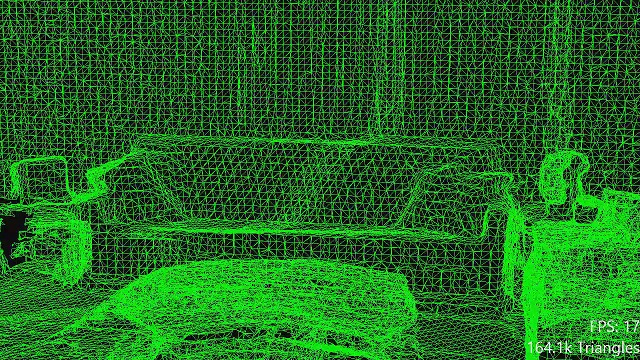
\includegraphics[width=\linewidth]{mesh.jpg}
    \caption{Mesh gemaakt door HoloLens spatial mapping algoritme}
    \label{fig:mesh}
\end{figure}

Zoals te zien op figuur \ref{fig:mesh} bevat de mesh redelijk veel detail over de ruimte, toch kan soms moeilijk om kleine details uit een mesh te krijgen \autocite{Evans2017}.

% TODO IMAGE Mesh
\subsection{Realisme}
Mixed reality zal één van de meest realistische VR technologieën zijn omdat deze de kracht van augmented en virtual reality bevat. Het is mogelijk om virtuele objecten in de echte wereld te plaatsen en om hier ook fysiek mee te reageren. Een extra vorm van realisme komt door het gebruik van occlusion. Dit is wanneer een virtueel object wordt geblokkeerd door een ander virtueel of zelfs fysiek object. Op deze manier zal de gebruiker nog meer het gevoel krijgen dat de virtuele wereld deel uit maakt van de echte \autocite{Evans2017}.

\subsection{Interactiviteit}
In tegenstelling tot augmented reality zal mixed reality wel rekening houden met de fysieke wereld. Op deze manier kan de gebruiker zijn handen gebruiken om met de virtuele wereld te communiceren. Hierdoor zijn er veel verschillende mogelijkheden om dit in een applicatie te implementeren.

Ook kan de headset gebruikmaken van een gewone \acrshort{6dof} controller op deze manier moet er geen rekening worden gehouden met welke gestures er ondersteund zijn.

\subsection{Bruikbaarheid}
Een mixed reality headset heeft, zolang deze niet aan het opgeladen is, ook geen kabel nodig en kan dus in het hele museum worden gebruikt alsook heeft deze geen externe sensoren nodig om aan room scale VR te doen. 

Het grote nadeel van een mixed reality headset is namelijk de prijs. Indien de applicatie ontwikkelt is voor thuisgebruik zal de doelgroep beperkt zijn, terwijl als het de bedoeling is om de applicatie te gebruiken in het museum zelf kan de kost wel nog oplopen.

% TODO ASK Uitleg gyropscoop? te ingewikkeld?
% TODO CONTENT Depth Camera
% TODO CONTENT Alternative devices? AR glasses? Future of?

\section{Conclusie Longlist}
Wanneer alle technologieën naast elkaar worden gelegd en er naar de drie variabelen wordt gekeken kan men zien dat elke technologie wel zijn voordelen heeft maar ook telkens zijn nadelen heeft. De `beste` technologie zal dus afhangen variëren van musea tot musea. 

Musea met veel geld zullen bijvoorbeeld kiezen om gebruik te maken van mixed reality om zo de meest interactieve en realistische ervaring te geven. Terwijl een stadsmuseum met een beperkt budget misschien eerder zal kiezen voor augmented reality om zo het ruime publiek dat zij over vloer krijgen aan te spreken. Het is ook voor deze reden dat augmented reality verder wordt besproken in de shortlist omdat deze de meest gemiddelde ervaring biedt.

Augmented reality biedt namelijk een goed niveau van realisme zolang dit goed geimplementeerd en wanneer de applicatie originele (maar passende) features bevat zal er ook tamelijk wat interactiviteit mogelijk zijn. Ook omdat alleen een smartphone nodig is zal een groot doelpubliek hebben.
\chapter{Shortlist frameworks ---GEKOZEN TECHNOLOGIE----}
\label{ch:shortlist}

In dit voorbeeld gebruik ik augmented reality

Eerst zal er een kleine inleiding worden gegeven over verschillende algoritmen die worden gebruikt binnenin augmented reality zoals plane detection, image detection... zodat de gebruiker goed weet wat deze termen betekenen.

Hierin worden de verschillende frameworks van de gekozen technologie uit de longlist overlopen en met elkaar vergeleken. Dit zal gebeuren door aan elk framework een score te geven gebaseerd op een lijst van must-haves en nice-to-haves. Deze zullen dan elk factor hebben die meer (must-have) of minder (nice-to-have) zal doorwegen in de score.

Vb must-have: moet op zoveel mogelijk devices draaien => aantal procent van de devices kan dan de score zijn voor deze must have
OF
een andere manier simpelere manier om dit voor te stellen zou a.h.v. sterren kunnen zijn. Bv 1 ster: draait op ioS, draait op android, draait op andere VR headsets...

Onderste secties zijn voorbeelden indien augmented reality wordt gekozen.

\section{8th Wall}
\section{ARCore}
\section{ARKit}
\section{Vuforia}
%%=============================================================================
%% Methodologie
%%=============================================================================

\chapter{Methodologie van het Experiment}
\label{ch:methodologie}

Om de kwaliteit van een augmented reality framework te beoordelen is het experiment in twee delen opgedeeld. Het eerste deel van het experiment zal gaan over hoe goed de frameworks de core van de applicatie kunnen implementeren. Elk framework zal dezelfde lijst met tien images. De bedoeling is dat elk framework zoveel mogelijk images probeert te herkennen. De gebruikte lijst met images kan u vinden in de bijlage. De lijst is opgebouwd uit vijf makkelijke afbeeldingen en vijf moeilijkere afbeeldingen. Om te weten wat een moeilijke of makkelijke afbeelding is gebruikt deze studie volgende criteria.

\begin{itemize}
    \item Veel features
    \item Geen repetitieve features
    \item Goed contrast
\end{itemize} 


Het tweede deel van het experiment zal gaan over de performance van elk framework. Dit wordt gedaan door FPS, RAM gebruik en batterij verbruik met elkaar te vergelijken. Omdat ieder framework gebruik maakt van andere API's moet voor elk van deze een soortgelijke applicatie worden voorzien. Deze applicatie zal een afbeelding herkennen aan hierop een 3d object tonen. Bij het klikken op dit object zal dit veranderen in een ander object. Het is de bedoeling dat bij het verliezen van de tracking van de afbeelding, en hierna terug tracken, het nieuwe object er nog steeds is en niet terug verandert is naar het oude.
%% TODO: Hoe ben je te werk gegaan? Verdeel je onderzoek in grote fasen, en
%% licht in elke fase toe welke stappen je gevolgd hebt. Verantwoord waarom je
%% op deze manier te werk gegaan bent. Je moet kunnen aantonen dat je de best
%% mogelijke manier toegepast hebt om een antwoord te vinden op de
%% onderzoeksvraag.

\chapter{Experiment}
\label{ch:experiment}

(TODO RAAMWERK) Indien een bepaald framework boven een bepaalde scoregrens ligt zal deze worden opgenomen in het experiment.
Voor het experiment zal een simpele applicatie worden ontwikkelt (touch op het scherm creëert een object) voor elk framework a.h.v. deze applicatie zullen dan volgende kenmerken worden gemeten:  FPS, memory usage.

Indien ik informatie vindt over het automatisch testen van AR applicaties zal deze ook hier terecht komen. Ook zal dit een invloed hebben op het uitvoeren van de experimenten. Als ik hierover bruikbare informatie vind zal ik deze ook gebruiken om het experiment meerdere malen uit te voeren i.p.v. het gelimiteerde aantal keren indien ik het manueel moet doen.

\section{Afbeeldingsherkenning}
Elk framework zal ook een lijst krijgen van 10 afbeeldingen om te kijken hoe goed hij verschillende afbeeldingen kan herkennen. Hier zal er ook worden gekeken van hoever hij deze kan herkennen!
Een conclusie waarom bepaalde afbeeldingen niet worden herkent kan hier ook in komen
\begin{figure}
    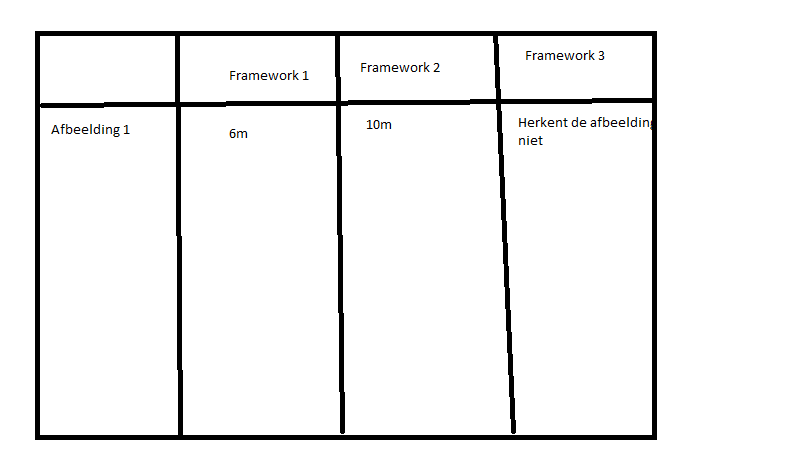
\includegraphics[width=\textwidth]{img/imgrex}\caption{Tabel aantal meter tot herkenning}\label{fig:imgrex}
\end{figure}

\section{FPS}\label{sec:fps}

Uit de data van beide frameworks blijkt het dat Vuforia maximum 60 FPS kan halen terwijl ARCore maar een maximum behaalt van 30 FPS. Het halen van een 60 FPS is redelijk onbelangrijk omdat vele Android Smartphones (vooral de iets oudere) nog geen 60 FPS camera ondersteunen. Het belangrijkste is een constant framerate behouden zonder veel grote FPS drops.

Om na te kijken of het framework een constant framerate kan behouden wordt de standaardafwijking gebruikt. Een kleine standaardafwijking wijst er namelijk op dat de datapunten weinig afwijken van het gemiddelde.

\begin{itemize}
    \item Vuforia: 1,60
    \item ARCore: 1.03
\end{itemize}

Beide frameworks hebben een kleine standaardafwijking wat er op wijst dat hun framerate redelijk (maar niet honderd procent) constant is. 

Een standaardafwijking groter dan nul wijst erop dat data niet constant is. Bij beide frameworks zijn er dus FPS drops aanwezig.

De grote van de FPS drops hebben een grotere impact op de ervaring dan de frequentie van de drops. Kleine drops van één tot twee frames hebben geen impact op de ervaring voor gebruiker omdat ze niet zichtbaar zijn. Daarom analyseert deze studie alleen maar de FPS drops die groter zijn dan tien frames.

\begin{itemize}
    \item Vuforia: 5
    \item ARCore: 3
\end{itemize}

\subsection{Analyse FPS Drops: Vuforia}

De oorsprong van de FPS drops bij Vuforia is makkelijk te achterhalen door naar het tijdstip te kijken wanneer ze voorkomen (zie tabel \ref{tbl:vuforiadrop}). In deze tabel is duidelijk te zien dat de drops altijd voorkomen bij het opstarten van de applicatie.

\begin{table}[]
    \begin{tabular}{@{}l|l|l|l|l|l@{}}
        & Drop 1   & Drop 2   & Drop 3   & Drop 4   & Drop 5   \\ \midrule
        Experiment         & 1        & 2        & 3        & 4        & 5        \\
        Tijdstip           & 1.003758 & 1.015506 & 1.013395 & 1.012443 & 1.012150 \\
        Frames per seconde & 33       & 34       & 32       & 34       & 34      
    \end{tabular}
    \caption{Oorsprong FPS drops experiment Vuforia}\label{tbl:vuforiadrop}
\end{table}

Op figuur \ref{fig:vuforiaTimeDrop} is te zien dat de framerate voor het verdere verloop van de applicatie stabiel blijft met hier en daar een kleine FPS (minder dan 10 frames) drop.

\begin{figure}
    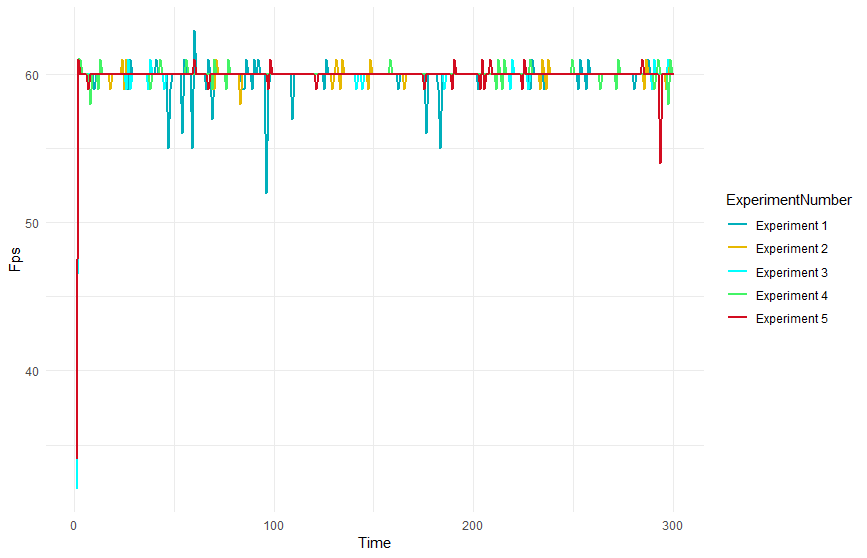
\includegraphics[width=\linewidth]{vuforiaTimeDrop.png}
    \caption{Vuforia: verloop van de FPS bij alle experimenten}
    \label{fig:vuforiaTimeDrop}
\end{figure}

\subsection{Analyse FPS Drops: ARCore}
Hoewel ARCore minder drops heeft dan Vuforia zijn ze wel veel groter (zie tabel \ref{tbl:arcoredrop}) in secties \ref{sec:memory} en \ref{sec:gameobjects} worden de oorzaken van deze drops verder besproken. Op figuur \ref{fig:arcoreTimeDrop} is te zien dat net zoals bij Vuforia de FPS bij alle experimenten redelijk consistent blijft doorheen de applicatie. Het grote verschil met Vuforia is dat de kleinere drops hoofdzakelijk geconcentreerd zijn in het begin (eerste 50 seconden) in plaats van verspreid te doorheen de looptijd van de applicatie. 

\begin{table}[]
    \begin{tabular}{@{}l|l|l|l@{}}
        & Drop 1    & Drop 2   & Drop 3    \\ \midrule
        Experiment         & 2         & 4        & 4         \\
        Tijdstip           & 218.63180 & 85.33646 & 250.73920 \\
        Frames per seconde & 8         & 7        & 10       
    \end{tabular}
    \caption{Oorsprong FPS drops experiment ARCore}\label{tbl:arcoredrop}
\end{table}

\begin{figure}
    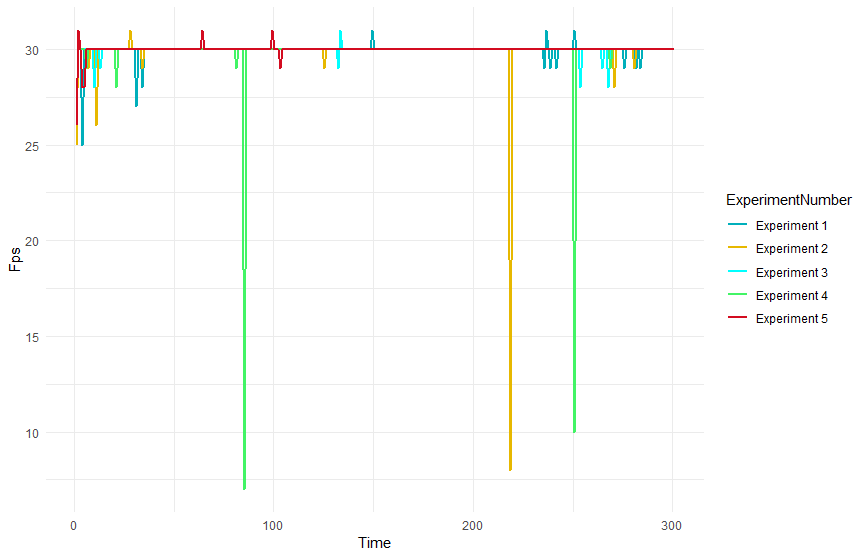
\includegraphics[width=\linewidth]{arcoreTimeDrop.png}
    \caption{ARCore: verloop van de FPS bij alle experimenten}
    \label{fig:arcoreTimeDrop}
\end{figure}

\section{RAM}\label{sec:memory}
Door de gemiddelden en standaardafwijkingen van het gereserveerde en geallorceerde RAM van beide frameworks te berekenen is het duidelijk dat de ARCore applicatie gemiddeld 4MB minder RAM verbruikt dan Vuforia. Dit is ook makkelijk te bewijzen door aan beide datasets een kolom toe te voegen waarin staat tot welk framework ze behoren en deze datasets samen te voegen. Op deze nieuwe dataset is een t-test uitgevoerd die als resultaat een p-waarde van 1 had wat erop wijst dat er een sterk verband is tussen het gekozen framework en het verbruikte RAM.

Het RAM-verbruik van Vuforia fluctueert ook veel meer dan ARCore, een standaardafwijking van 4.5MB tegenover 0.06MB. Dit is ook te bewijzen door een t-test uit te voeren op een nieuwe kolom die het vorige RAM - het huidige RAM bevat. Het resultaat van deze test was een p-waarde van 0.7419 wat aantoont dat het RAM-verbruik van ARCore inderdaad stabieler is.

Wanneer het gereserveerde RAM stijgt is het ook logisch dat gealloceerde RAM stijgt. Een applicatie gaat niet meer RAM reserveren tenzij deze meer RAM nodig heeft. Dit is bewezen door het correlatiecoëfficiënt van gereserveerd tegenover gealloceerd RAM en het correlatiecoëfficiënt van de stijging in gereserveerd RAM tegenover de stijging in gealloceerd RAM te berekenen. In tabel \ref{tbl:ramcor} is te zien dat bij beide frameworks hier een volstrekt verband is.

\begin{table}[]
    \begin{tabular}{@{}l|l|l@{}}
        & Gereserveerd tegenover gealloceerd & Stijging gereserveerd tegenover stijging gealloceerd \\ \midrule
        Vuforia & 0.9987308                          & 0.9496204                                            \\
        ARCore  & 0.9981332                          & 0.9999941                                           
    \end{tabular}
 \caption{De correlatiecoëfficiënten gereserveerd en gealloceerd RAM tonen een duidelijk verband}
\end{table}

\subsection{Correlatie RAM en FPS}
Zoals er eerder vermeld in sectie \ref{sec:fps} kampen beide frameworks met FPS drops. Om deze FPS drops te verklaren 


\section{Conclusie best scorend framework}
Hierin komt de conclusie over het best scorend framework en waarom deze de best scorende is. Hierin zal ook rekening worden gehouden met de score van het vorige hoofdstuk!
\chapter{Uitwerken prototype ---GEKOZEN FRAMEWORK---}
\label{ch:prototype}

Dit hoofdstuk bevat een omschrijving van het uitgewerkte prototype. Het prototype bestaat uit verschillende grote delen die elk besproken worden in een aparte sectie.

\section{Unity Asset Store}
Unity beschikt over een Asset Store die developers, designers en zelfs muzikanten kunnen gebruiken om hun werk te delen met anderen. De assets op deze store kunnen andere developers dan gebruiken in hun projecten. Voor de ontwikkeling van het protype zijn volgende assets gebruikt:

\begin{itemize}
    \item ZoneUI \autocite{MichskyZone}
    \item Clean Title Transitions \autocite{MichskyTitle}
\end{itemize}

\section{Hoofdmenu}
Wanneer de gebruiker de applicatie opstart komt hij op de hoofdpagina (zie figuur \ref{fig:prototypeUi}) terecht. Op deze pagina heeft hij verschillende opties waaruit hij kan kiezen. Als het de gebruiker zijn eerste keer is dat hij de applicatie gebruikt zullen alleen de opties 'Nieuw Levensverhaal' en 'Oud Levensverhalen bekijken' beschikbaar zijn. Indien de gebruiker toch al eens de applicatie heeft opgestart kan hij verder doen met zijn recentste levensverhaal of kiezen uit één van zijn niet voltooide levensverhalen. 

Vanuit het hoofdmenu heeft de gebruiker ook nog de optie om naar de instellingenpagina te gaan of naar zijn profielpagina. Op de gebruiker zijn profiel staan verschillende weetjes zoals het aantal deelgenomen levensverhalen, voltooide raadsels en ontdekte schilderijen. Ook heeft de gebruiker een level dat berekent is aan de hand van deze variabelen. Het behalen van een bepaald level is momenteel puur aesthetic en zit in de applicatie om de gebruiker een gevoel van trots en prestatie te geven.

\begin{figure}
    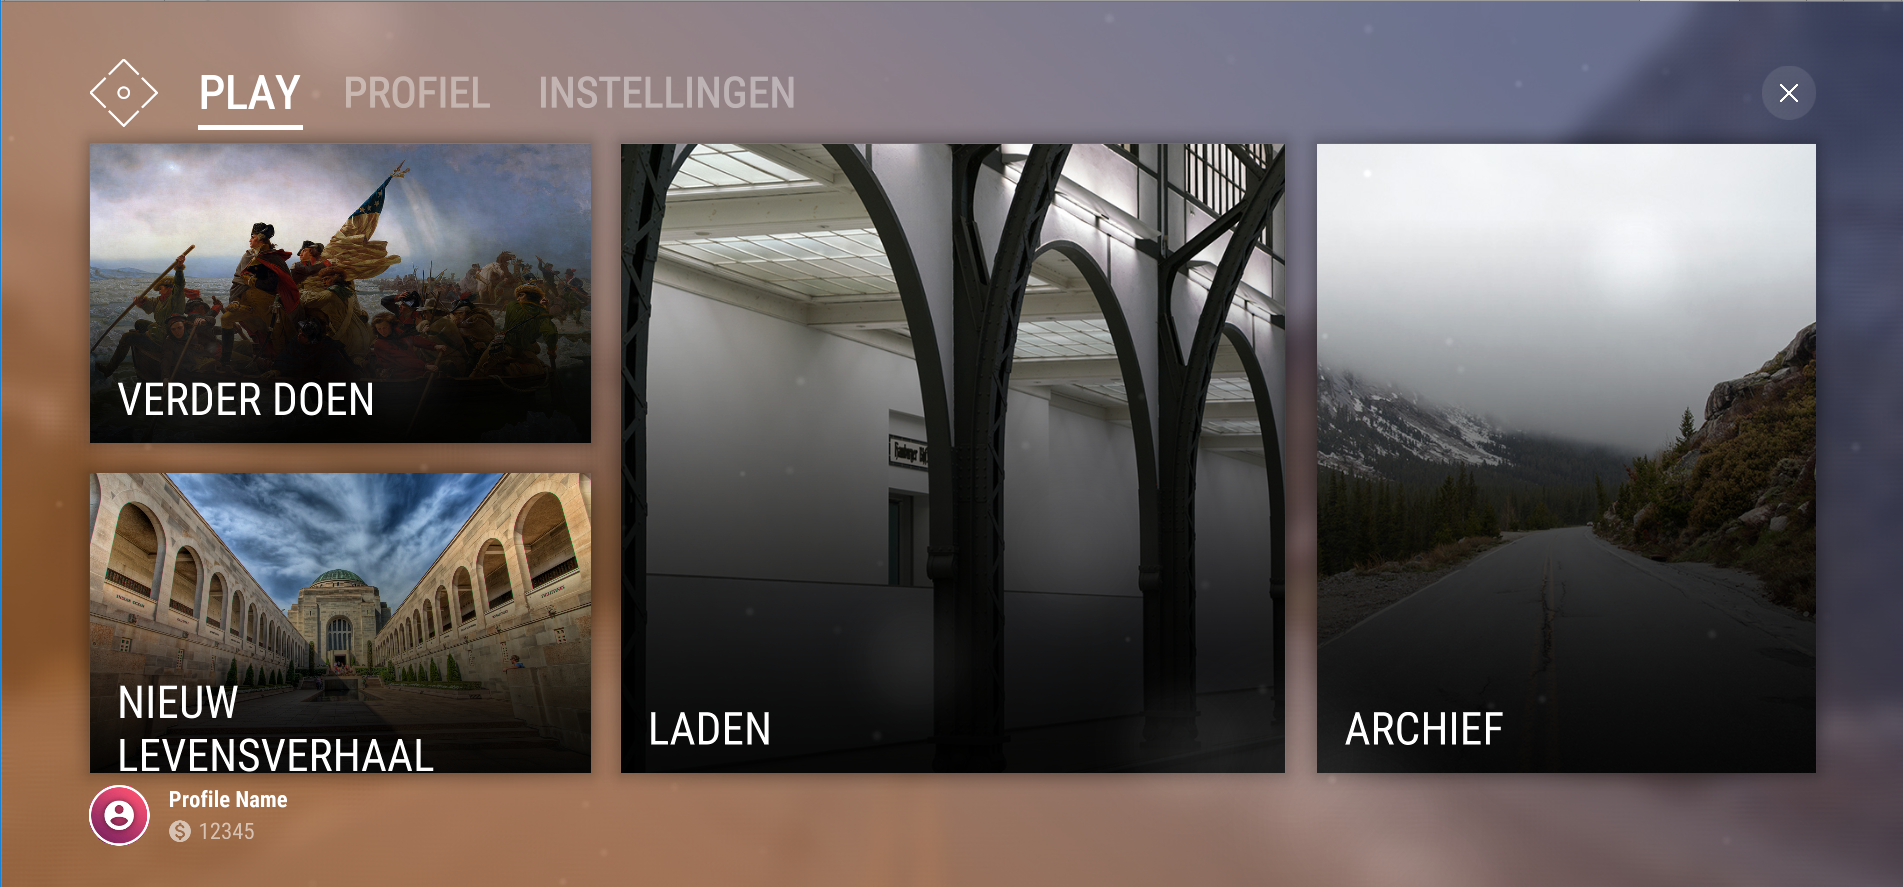
\includegraphics[width=\linewidth]{prototypeUi.png}
    \caption{Het hoofdmenu}
    \label{fig:prototypeUi}
\end{figure}
% + 1 If you get the reference

\section{Nieuw Levensverhaal Starten}
De gebruiker heeft de optie om een nieuw levensverhaal op te starten. Wanneer hij voor deze opties kiest krijgt hij een lijst van alle beschikbare levensverhalen. Deze lijst is niet hardcoded in de applicatie. Bij het opstarten zal de applicatie de lijst ophalen van een backendserver. Wanneer de gebruiker kiest voor levensverhaal moet de applicatie wel nog de concrete data ophalen van dit levensverhaal. Deze data is van het JSON datatype en bevat:

\begin{enumerate}
    \item Informatie over het levensverhaal
    \item Raadsels gelinkt aan het levensverhaal
    \item De benodigde afbeeldingen
\end{enumerate}

Door het levensverhaal op deze manier op te slaan is het makkelijk voor musea om nieuwe verhalen te creëren via een webinterface en deze direct beschikbaar te stellen voor de gebruiker. Omdat de afbeeldingen niet op voorhand beschikbaar zijn moet ARCore data image database wel 'at runtime' creëren. Het toevoegen van een image 'at runtime' duurt ongeveer 30ms (wat niet lang is) en zolang het creëren van deze database op een ander thread gebeurt kan de gebruiker nog steeds de UI gebruiken.

\subsection{Verloop van een Levensverhaal}
Wanneer het levensverhaal geladen is kan de gebruiker aan de slag gaan. De gebruiker krijgt het eerste kunstwerk te zien dat hij moet inscannen. Bij het inscannen van het kunstwerk krijgt de gebruiker dan wat extra informatie over het kunstwerk en de persoon waarover het gaat. Ook krijgt hij het volgende kunstwerk te zien dat hij moet inscannen. Bij het inscannen van het volgende kunstwerk kunnen er nu meerdere dingen gebeuren:

\begin{enumerate}
    \item Het nieuwe kunstwerk is beschikbaar
    \item Het nieuwe kunstwerk is nog niet beschikbaar en de gebruiker moest eerst een raadsel oplossen
\end{enumerate}

In het eerste geval gaat de applicatie gewoon verder zoals bij het eerste kunstwerk. Bij het tweede geval moet de gebruiker iets extra doen om het volgende kunstwerk te kunnen scannen. Deze raadsels kunnen van verschillende vormen waaronder:

\begin{enumerate}
    \item Antwoorden van een vraag
    \item Opzoek gaan naar een item in een voorafgaand kunstwerk
    \item Opzoek gaan naar een item in het huidige kunstwerk
\end{enumerate}

Deze cyclus blijft verder gaan tot de gebruiker het hele levensverhaal heeft ontdekt.

\section{Lijst van Levensverhalen}
In dit scherm bevinden zich alle levensverhalen die ooit hebben bestaan zelf als de gebruiker er niet aan heeft meegedaan. Op deze manier gaat het werk van het museum nooit verloren. De gebruikers kunnen hier een levensverhaal selecteren en de informatie over de kunstwerken lezen. Ook is er de optie om zelf de schilderijen af te drukken waardoor de gebruikers ook de mogelijkheid hebben om bij hun thuis de tentoonstelling uit te voeren.
% Voeg hier je eigen hoofdstukken toe die de ``corpus'' van je bachelorproef
% vormen. De structuur en titels hangen af van je eigen onderzoek. Je kan bv.
% elke fase in je onderzoek in een apart hoofdstuk bespreken.

%\input{...}
%\input{...}
%...

%%=============================================================================
%% Conclusie
%%=============================================================================

\chapter{Conclusie}
\label{ch:conclusie}

%% TODO: Trek een duidelijke conclusie, in de vorm van een antwoord op de
%% onderzoeksvra(a)g(en). Wat was jouw bijdrage aan het onderzoeksdomein en
%% hoe biedt dit meerwaarde aan het vakgebied/doelgroep? Reflecteer kritisch
%% over het resultaat. Had je deze uitkomst verwacht? Zijn er zaken die nog
%% niet duidelijk zijn? Heeft het onderzoek geleid tot nieuwe vragen die
%% uitnodigen tot verder onderzoek?

Net zoals bij andere informaticaontwikkelingen zien we dat virtual reality ook vaak te kampen heeft met te moeten wachten op een andere hard- of software. Zelfs zoiets simpel als augmented reality moet vaak rekening houden met een groot verschil van hardware binnenin smartphones. Virtual en Mixed Reality hebben dan weer veel te dure prijzen omdat het ontwikkelingsproces van deze nog niet geoptimaliseerd is. Het daarom moeilijk te zeggen wat de toekomst juist gaat inhouden voor Virtual Reality wel zien we dat grote bedrijven hiermee experimenteren en al goede resultaten boeken. Echter zal het een hele tijd duren vooraleer deze leuke snufjes betaalbaar zijn voor consumenten of zelfs musea. Dit zorgt wel niet voor dat het onmogelijk is om immersive ervaringen te maken, het kost alleen net iets meer moeite van developers en designers om een applicatie te ontwikkelen die het gepaste niveau van teleprescence opkweekt met de beperkte tooling.

Musea zitten momenteel ook met het probleem dat deze niet echt beschikken over een infrastructuur om de vr-applicaties in te draaien. Het is daarom eigenlijk wel logisch dat augmented reality als beste technologie naar voren komt omdat er hiervoor weinig infrastructuur nodig is. De opkomst van 5G zou vele van deze problemen wel moeten oplossen. De snelheid van 5G is veel sneller dan de huidige verbindingen en zou toestaan om vele software volledig in de cloud te laten draaien waardoor headsets en smartphones de taak van het mappen van een ruimte kunnen overlaten aan de cloud. Dit lost ook meteen latency luik van virtual reality sickness op zoals beschreven in sectie \ref{sec:medical}\autocite{Bastug2017}.

Voor het implementeren van de applicatie maakte het framework niet zoveel uit. Meeste AR frameworks beschikken over dezelfde features waardoor de keuze vrij is. Bij de frameworks gespecialiseerd op één bepaald doelgebied (Vuforia met image recognition en 8th Wall met browserondersteuning) is het wel duidelijk dat deze lager scoren in de andere doelgebieden. De toekomst voor deze frameworks ziet er rooskleurig uit. Tijdens het onderzoek heeft 8th Wall Web ondersteuning gekregen voor het herkennen van images terwijl ARCore nu bewegende images kan blijven tracken.



%%=============================================================================
%% Bijlagen
%%=============================================================================

\appendix

%%---------- Onderzoeksvoorstel -----------------------------------------------

\chapter{Onderzoeksvoorstel}

Het onderwerp van deze bachelorproef is gebaseerd op een onderzoeksvoorstel dat vooraf werd beoordeeld door de promotor. Dat voorstel is opgenomen in deze bijlage.

% Verwijzing naar het bestand met de inhoud van het onderzoeksvoorstel
%---------- Inleiding ---------------------------------------------------------

\section{Introductie} % The \section*{} command stops section numbering
\label{sec:introductie}

Virtual reality wordt momenteel al op veel verschillende manieren gebruikt in verscheidende sectoren. Dit onderzoek wil nagaan of het ook mogelijk is om virtual reality of augmented reality op een goede manier te gebruiken om het levensverhaal van een persoon te vertellen. Indien dit effectief mogelijk is zal er een long- en shortlist worden gemaakt om de verschillende frameworks en technologieën met elkaar te vergelijken. Aan de hand van de shortlist kan er dan worden gekeken welke technologie de beste is. Met beste wordt hier niet de meest performante bedoeld maar eerder welk prototype het meest toepasbaar is in de gekozen sector.

%---------- Stand van zaken ---------------------------------------------------

\section{State-of-the-art}
\label{sec:state-of-the-art}

Momenteel zijn er al verschillende onderzoeken geweest naar het toepassen van virtual reality in verscheidende sectoren. Ook is er al onderzoek gedaan naar het gebruik van virtual reality in de sectoren die in dit onderzoek aan bod komen, namelijk psychologie \autocite{Wilson2014} en musea \autocite{Jung2016}. Maar geen enkel van deze onderzoeken gaat specifiek over het vertellen van een levensverhaal in virtual reality.
Bij het opzetten van een applicatie in VR is het heel belangrijk dat er rekening wordt gehouden met de sociale aanwezigheid \autocite{Jung2016}. Hiermee wordt er bedoeld dat hoe minder de gebruiker het doorheeft dat hij in een virtuele wereld zit hoe beter de ervaring zal zijn.   

Uit een onderzoek in de psychologie blijkt dat virtual reality positieve effecten kan hebben, maar dat er ook opgepast moet worden voor bepaalde bijeffecten indien de ervaring niet immersief genoeg is \autocite{Wilson2014}.

Bij het toepassen van virtual reality in musea moet er een duidelijk onderscheid worden gemaakt tussen virtual reality en augmented reality. Hoewel virtual reality (met bewegingsvrijheid) een heel immersieve ervaring geeft, zullen veel gebruikers en musea toch augmented reality verkiezen \autocite{Kersten2017}. Dit is omdat het gebruik van AR gepaard zal gaan met een fysiek bezoek aan het museum. Natuurlijk is het ook belangrijk hierbij dat de ervaring leerrijk is. Uit het onderzoek van Davies Andrew G.\textcite{Davies2018} blijkt dat VR inderdaad kan gebruikt worden om iets bij te leren.

Veel mensen worden afgeschrikt door VR ontwikkeling en gebruik door de kostprijs. Alhoewel dit nu een kleiner probleem is door de opkomst van nieuwe VR frameworks zoals WebVR die het ontwikkelen van VR goedkoper maken \autocite{Dibbern2018}. Ook omdat nu bijna alle smartphones uitgerust zijn met de mogelijkheid om VR te tonen is het gebruik van deze applicaties toegankelijker.
% Voor literatuurverwijzingen zijn er twee belangrijke commando's:
% \autocite{KEY} => (Auteur, jaartal) Gebruik dit als de naam van de auteur
%   geen onderdeel is van de zin.
% \textcite{KEY} => Auteur (jaartal)  Gebruik dit als de auteursnaam wel een
%   functie heeft in de zin (bv. ``Uit onderzoek door Doll & Hill (1954) bleek
%   ...'')



%---------- Methodologie ------------------------------------------------------
\section{Methodologie}
\label{sec:methodologie}

Tijdens het onderzoek zal er worden gekeken naar de verschillende manieren om Virtual en Augmented Reality te ontwikkelen waaronder WebVR (A-Frame), Unity en Unreal Engine. Maar ook naar de verschillende soorten ervaringen zoals: Augmented Reality, 360\textdegree\space en VR met en zonder bewegingsvrijheid. 
Om te bepalen welke technologie de beste is zal er eerst een longlist worden opgesteld met de mogelijke technologieën. Vanuit deze longlist zal er dan een shortlist worden opgesteld met de meeste belovende technologieën. Dit zijn degene die realistisch zouden zijn om te implementeren (huidige vooruitgang technologie en beperking budget). Aan de hand van elke technologie in de shortlist wordt er dan gekeken hoe goed de ervaring is voor de gebruiker. Dit zal worden gemeten aan de hand van functionele en niet-functionele requirements waaronder: de instapkost, de interactiviteit voor de gebruiker en bruikbaarheid binnenin de sector.


%---------- Verwachte resultaten ----------------------------------------------
\section{Verwachte resultaten}
\label{sec:verwachte_resultaten}

Als resultaat wordt er een analyse verwacht van de verschillende technologieën die hun waarde (instapkost, interactiviteit en bruikbaarheid in de realiteit) met elkaar vergelijkt. Uit deze analyse zal het dan mogelijk zijn om af te leiden welke ervaring de beste is voor de gekozen use case. De beste technologie zal dan verder ontwikkeld worden om zo een beter beeld te hebben over de volledige ervaring.

%---------- Verwachte conclusies ----------------------------------------------
\section{Verwachte conclusies}
\label{sec:verwachte_conclusies}

Er wordt verwacht dat uit de analyse van de verschillende technologieën gaat blijken dat hoe hoger de instapkost is hoe hoger de interactiviteit zal zijn. Dit betekent niet dat het prototype met de hoogste instapkost en dus hoogste interactiviteit ook de hoogste bruikbaarheid zal hebben. Er wordt verwacht dat augmented reality de hoogste bruikbaarheid zal hebben door de lage instapkost maar dat de interactiviteit wel beperkt zal zijn. Een echte volledige virtual reality applicatie zal dan veel interactiever zijn maar ook wel de hoogste instapkost hebben. Alsook wordt er verwacht dat de ontwikkeling van een applicatie met WebVR het makkelijkste gaat zijn door zijn simpliciteit en gelijkenis met HTML. De beste technologie zal dus diegene zijn die een goede balans kan vinden tussen instapkost en interactiviteit.



%%---------- Andere bijlagen --------------------------------------------------
% TODO: Voeg hier eventuele andere bijlagen toe
%\input{...}

%%---------- Referentielijst --------------------------------------------------

\printbibliography[heading=bibintoc]
%\addcontentsline{toc}{chapter}{\textcolor{maincolor}{\IfLanguageName{dutch}{Bibliografie}{Bibliography}}}

\end{document}
